\documentclass[../../main.tex]{subfiles}
% 
\begin{document}
\chapter{Častice a ich vzájomné interakcie}
\section{Zadanie}
Častice a ich vzájomné interakcie, Interakcie medzi elementárnymi časticami, Vlastnosti elementárnych častíc, Klasifikácia elementárnych častíc, Hadróny, Leptóny, Antičastice, Symetrie a zákony zachovania, Štandardný model, Zákony zachovania energie a hybnosti, Súradnicové sústavy v subjadrovej fyzike, Transformácie kinematických veličín medzi sústavami, Mandelstamové premenné, Kinematické premenné – rapidita. pseudorapidita, Feynmanova premenná, Bjorkenova premenná

%OOOOOOOOOOOOOOOOOOOOOOOOOOOOOOOOOOOOOOOOOOOOO
%OOOOOOOOOOOOOOOOOOOOOOOOOOOOOOOOOOOOOOOOOOOOO
%OOOOOOOOOOOOOOOOOOOOOOOOOOOOOOOOOOOOOOOOOOOOO
\section{Štandardný model}
\subsection{História}
V roku 1960 navrhol Sheldon Glashow teoretickú možnosť ako skombinovať elektromagnetickú a slabú interakciu do jednotnej teórie. O sedem rokov neskôr doplnili Steven Weinberg a Abdus Salam navrhnutý teoretický model o Higgsov mechanizmus, ktorý priamo determinuje hmotnosti elementárnych častíc popísaných v rámci štandardného modelu. Špeciálne ide hlavne o hmotnosti W a Z bozónov a fermiónov. Higgsov mechanizmus takisto vysvetľuje, akým spôsobom získavajú hmotnosť kvarky a leptóny.

Po objave slabých neutrálnych prúdov v CERN-e, spôsobených výmenou Z bozónov sa elektroslabá teória stala široko akceptovanou. Glashow, Salam a Weinberg, tvorcovia tejto teórie, následne dostali v roku 1979 Nobelovú cenu za fyziku. Neskôr, v 1981 boli experimentálne objavené bozóny W a Z. Experimentálne boli určené ich hmotnosti, pričom tieto hmotnosti boli v dobrej zhode s predpoveďami poskytnutými Štandardným modelom. Teória silnej interakcie získala svoju modernú podobu v 70. rokoch, kedy experimenty potvrdili, že hadróny sú zložené z nabitých kvarkov.

\subsection{Prehľad}
Štandardný model fyziky častíc je zjednotený súbor teoretických poznatkov zahrňujúci väčšinu známych elementárnych častíc. V rámci modelu je možné zjednoteným spôsobom ( zjednotenou matematickou formuláciou ) popísať tri zo štyroch fundamentálnych interakcií: silnú, slabú, a elektromagnetickú. Štandardný model predstavuje relativistickú kvantovú teóriu vyhovujúcu zároveň princípom špeciálnej teórie relativity i kvantovej mechaniky. Gravitačná interakcia a teda ani všeobecná teória relativity nie sú v modeli zahrnuté. Fundamentálnymi objektmi vystupujúcimi v tejto teórii sú polia v časopriestore. Štandardný model bol vypracovávaný postupne. Jeho základy boli položené začiatkom 20. storočia. Súčasná formulácia bola dokončená po experimentálnom potvrdení existencie kvarkov. Táto teória je v dobrom súlade so súčasnými experimentálnymi údajmi. Zahrňuje však 18 voľných parametrov, ktorých hodnotu nepredpovedá. Hodnota týchto parametrov je určená výhradne na základe experimentálnych výsledkov. Nepopisuje taktiež gravitáciu, tmavú hmotu či tmavú energiu.
 
Štandardný model je kalibračná teória silných (SU(3)) a elektroslabých (SU(2) $\times$ U(1)) interakcií s kalibračnou grupou nazývanou tiež Štandardný model symetrickej grupy SU(3) $\times$ SU(2) $\times$ U(1). V nasledujúcej časti si povieme o elementárnych časticiach a interakciách medzi nimi.

\section{Elementárne častice a ich klasifikácia} 
Pod pojmom elementárna častica alebo fundamentálna častica rozumieme časticu, ktorej subštruktúra je neznáma, a teda nie je známe, či je daná častica zložená z  menších častíc. Tieto častice môžu byť rozdelené do dvoch skupín: elementárne fermióny a bosóny.
\subsection{Elementárne fermióny} 
Do tejto skupiny patria kvarky a leptóny, ktoré tvoria hmotu okolo nás preto ich môžme nazvať aj časticami hmoty. Rozdelenie týchto častíc je zobrazené v tabuľke (\ref{sf1:fig:Tabulka_fermionov}).
\begin{figure}[!h]
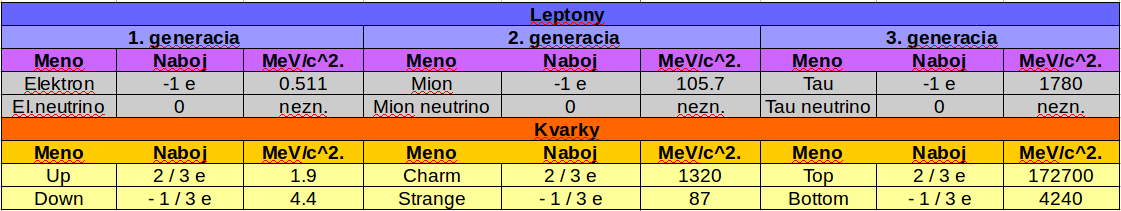
\includegraphics[width=1.0\textwidth]{Vlastnosti_tabulka.png}
\caption{Tabuľka fermiónov.}
\label{sf1:fig:Tabulka_fermionov}
\end{figure}

Všetky elementárne fermióny sú častice so spinom (1/2), antisymetrickou vlnovou funkciou, spĺňajúce Pauliho vylučovací princíp a ich správanie určuje Fermi-Diracovo rozdelenie, ktoré vyzerá nasledovne
\begin{equation}
f(\epsilon_i)=\frac{1}{e^{(\epsilon_i-\mu)/kT}+1},
\end{equation}
kde $k$ je Boltzmanová konštanta, $T$ je absolútna teplota, $\epsilon_i$ je energia jedno-časticového stavu $i$ a $\mu$ je celkový chemický potenciál.

Nabité \textbf{leptóny} ($e^{-}$, $\mu^{-}$, $\tau^{-}$) interagujú elektromagnetickou a slabou interakciou, zatiaľ čo neutrálne leptóny (neutrína) interagujú iba slabou interakciou. Leptóny neinteragujú silnou interakciou!

\textbf{Kvarky} interagujú silnou, slabou a elektromagnetickou interakciou. Každý kvark nesie jeden z troch farebných nábojov silnej interakcie (green, red, blue). Izolované kvarky neboli nikdy v prírode pozorované a vyskytujú sa len vo viazaných stavoch zvaných \textbf{hadróny}, ktoré majú neutrálny farebný náboj. Niektoré hadrónov sú takmer stabilné a niektoré (známe ako rezonancie) majú extrémne krátku životnosť. Stupeň stability závisí hlavne od hmotnosti hadrónu. Hadróny môžme rozdeliť na baryóny a mezóny. 

\begin{itemize}
\item \textbf{Baryóny} sú zložené častice, ktoré obsahujú 3 kvarky a majú polovičný spin, napr.(proton-uud, neutron-udd, $\Lambda$-uds). Baryón, ktorý obsahuje jeden alebo viac strange kvarkov, ale žiadny charm, bottom alebo top kvark, sa nazýva hyperón. Keďže silné interakcie si zachovávajú zvláštnosť (strangeness), hyperóny sa nemôžu rozpadnúť silnou interakciou avšak zučasťnúju sa silnej interakcie (to znamená, že môžu vzniknúť silnou interakciou). Rozpadajú sa niekoľko-násobnou slabou interakciou, ktorá mení ich strangeness, poväčšine na protón alebo neutrón (slabá interakcia podivnosť nezachováva).
\item \textbf{Mezóny} sú zložene z jedného kvarku a jedného antikvarku a výsledný mezón musí byť bezfarebný. Všetky mezóny sú nestabilné, pričom najdlhšia životnosť trvá len niekoľko stotín mikrosekúnd. Nabité mezóny sa rozpadajú na elektróny a neutrína (ako môžu sa rozpadnúť aj na iné mezóny ale tie sa potom tiež rozpadnú až to väčšinou skončí na leptonóch). Nenabité mezóny sa môžu rozpadnúť aj na fotóny. Obe tieto rozpady naznačujú, že farebný náboj už nie je vlastnosťou vedľajších produktov. Rozlišujú sa mezóny skalárne (spiny kvarku a antikvarku sú orientovane opačne, takže výsledný spin mezónu je 0) a mezóny vektorové (spin kvarku a antikvarku majú rovnaký smer, takže výsledný spin mezónu je 1). Mezóny sa zaraďujú medzi bozóny, keďže majú celočíselný spin avšak, nie medzi elementárne bozóny. 
\end{itemize}
\subsection{Elementárne bozóny}
Sú to častice, ktoré sprostredkúvajú základne interakcie; fotón pre elektromagnetickú interakciu, bozóny $W^{\pm}$, $Z^0$ pre slabú interakciu a gluóny pre silnú interakciu. Tieto častice majú celočíselný spin, symetrickú vlnovú funkciu, nespĺňajú Pauliho vylučovací princíp a ich správanie je riadene Bose-Einsteinovou štatistikou, ktorá ma nasledujúci tvar
\begin{equation}
f(\epsilon_i)=\frac{1}{e^{(\epsilon_i-\mu)/kT}-1}.
\end{equation}
Do tejto skupiny patrí aj Higgsov bozón, ktorý ma nulový spin.

\section{Fundamentálne interakcie}
Ešte než prejdeme k jednotlivému popisu jednotlivých interakcii, uvedieme tabuľku, v ktorej sú základne charakteristiky fundamentálnych interakcii, viď tabuľku \ref{sf1:fig:Tabulka_interakcie}
\begin{figure}[!h]
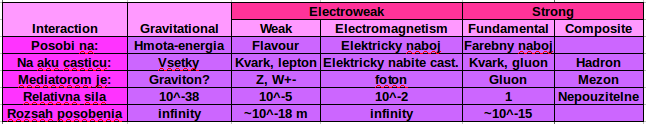
\includegraphics[width=1.0\textwidth]{Tabulka_interakcie.png}
\caption{Tabuľka interakcii.}
\label{sf1:fig:Tabulka_interakcie}
\end{figure}
\subsection{Elektromagnetická interakcia}
Prvou interakciou, ktorou sa budeme zaoberať, je elektromagnetická interakcia, ktorá pôsobí medzi časticami s nenulovým elektrickým nábojom. Mediátorom tejto interakcie je fotón, čo je vektorová častica (spin = 1).

Opis tejto interakcie začneme najprv z klasického hľadiska. V klasickom elektromagnetizme sa elektromagnetické pole riadi známymi Maxwellovými rovnicami
\begin{equation}
\begin{gathered}
\nabla \cdot \vec{E} = \frac{\rho}{\epsilon_0}\\
\nabla \cdot \vec{B} = 0\\
\nabla \times \vec{E}=-\frac{\partial \vec{B}}{\partial t}\\
\nabla \times \vec{B}= \mu_0 \vec{j}+\mu_0\epsilon_0\frac{\partial \vec{E}}{\partial t}
\end{gathered}
\end{equation} 
Prvá rovnica opisuje, ako sú elektrické polia vyvolané nábojmi. Druhá rovnica hovorí, že neexistuje nič také ako magnetický monopol. Tretia rovnica opisuje indukciu elektrických polí zmenou magnetických polí a štvrtá rovnica opisuje generovanie magnetických polí elektrickými prúdmi a indukciu magnetických polí časovou zmenou elektrických polí.

Z druhej a tretej Maxwellovej rovnice sa navyše dá ukázať, že polia $\vec{E}$ a $\vec{B}$ môžu byť prepísané následovne 
\begin{equation}
\begin{gathered}
\vec{B} = \nabla \times \vec{A}\\
\vec{E} = -\nabla\varphi-\frac{\partial}{\partial t}\vec{A},
\end{gathered}
\end{equation}  
kde funkcia $\vec{A}$ sa nazýva vektorový elektromagnetický potenciál a funkcia $\varphi$ je skalárny elektromagnetický potenciál. Skalárny a vektorový potenciál sú určené hustotami elektrického náboja a prúdu prostredníctvom rovníc, ktoré dostaneme zo zvyšných dvoch Maxwellových rovníc, keď do nich dosadíme $\vec{B}$ a $\vec{E}$ vyjadrené cez dane potenciály. Čo je však dôležitejšie je to, že tieto potenciály nie sú určene jednoznačne. A tak môžme z potenciálu $\vec{A}$ prejsť na potenciál 
\begin{equation}
\vec{A} \rightarrow \vec{A}+grad(\Lambda).
\end{equation}
Toto môžme urobiť preto lebo rotácia gradientu akejkoľvek vektorovej funkcie je vždy nula, takže naše $\vec{B}$ sa v konečnom dôsledku vôbec nezmení. Následne aby sa nezmenil ani skalárny potenciál tak aj ten musí prejsť z $\varphi$ na
\begin{equation}
\varphi \rightarrow \varphi -\frac{\partial}{\partial t}\Lambda.
\end{equation}
Touto transformáciou poli sa nezmení ani $\vec{B}$ ani $\vec{E}$. Uvedená transformácia elektromagnetických potenciálov (oboch súčasne!) sa nazýva \textbf{kalibračná transformácia}.

Prečo sme to ale vlastne cele robili a zaviedli sme takéto potenciály? Odpoveďou napríklad je, že kvantová mechanika častice v elektromagnetickom poli je opísaná Schrodingerovou rovnicou, v ktorej vystupujú elektromagnetické potenciály a nie elektromagnetické polia. Nahradenie potenciálov poliami by tu bolo značne komplikovane a neprirodzene. Navyše kvantová teória samotného elektromagnetického poľa, tzv. kvantová elektrodynamika, je založená na tzv. kvantovaní klasickej teórie. K tomuto kvantovaniu je potrebne mat sformulovanú klasickú elektrodynamiku v lagrangeovskom alebo hamiltonovskom formalizme. Pre oba tieto formalizmy su elektromagnetické potenciály oveľa vhodnejšie a prirodzenejšie ako elektromagnetické polia.

Problémy klasického elektromagnetizmu nastali keď Einstein publikoval teóriu fotoelektrického javu, v ktorej predpokladá, že svetlo se nešíri ako vlnenie elektromagnetického poľa, ale môže existovať vo forme častíc, diskrétnych kvánt, neskor nazývaných fotóny. Einsteinová teória fotoelektrického javu bola v súlade s predstavami, ktoré sa objavili v navrhnutom riešení Maxa Plancka v roku 1900. Vo svojej práci Planck predpokladal, že elektromagnetické vyžarovanie telies prebieha cez diskrétne kvantá, čo vedie ku konečnej celkovej energii. Tato predstava bola v priamom protiklade s klasickým pohľadom na svetlo ako spojitú vlnu. Plancková a Einsteinová teória následne viedla ku kvantovej mechanike, ktorá bola formulovaná v roku 1925. Na jej základe bola okolo roku 1940 dokončená nová kvantovo-mechanická teória elektromagnetizmu; kvantová elektrodynamika (QED) a je jednou z najpresnejších fyzikálnych teórii.

\textbf{Kvantová elektrodynamika} je náuka o pohybe elektrických nábojov (nabitých telies) v obecne premenných elektromagnetických poliach. Klasická elektrodynamika študuje elektrodynamické interakcie medzi makroskopickými telesami, kvantová elektrodynamika interakcie medzi mikro-objektmi. QED popisuje interakciu žiarenia s hmotou (fotoelektrický jav, Comptonov rozptyl, brzdné žiarenie), elektromagnetické interakcie medzi nabitými elementárnymi časticami prostredníctvom fotónov. Kvantová elektrodynamika vznikla ako teória interakcie elektromagnetického poľa a poľa popisujúceho elektróny a pozitróny.

A poďme teraz na samotný matematicky aparát QED. Tento bude trochu dlhší ako tie ďalšie dva a to len preto aby sme si demonštrovali silu už spomenutých kalibračných transformácii. Začneme veľmi z ľahká a to tým, že si napíšeme Diracov lagrangian pre diracovú voľnú časticu (kde $c$=$h$=1).
\begin{equation}
\mathcal{L}_D=\bar{\psi}(i\gamma^{\mu}\partial_{\mu}-m)\psi
\end{equation}
Pomocou Euler–Lagrangeovej rovnice pohybu pre pole, ktorá ma tvar
\begin{equation}
\partial_{\mu}\bigg(\frac{\partial \mathcal{L}}{\partial(\partial_{\mu}\psi)}\bigg)-\frac{\partial\mathcal{L}}{\partial\psi}=0,
\end{equation}
sme schopný dostať Diracovú rovnicu v tvare
\begin{equation}
(i\gamma^{\mu}\partial_{\mu}-m)\psi=0.
\end{equation}
Toto je pohybová rovnica pre voľné elektróny. V prípade pozitrónu by sme dostali
\begin{equation}
\bar{\psi}(i\gamma^{\mu}\partial_{\mu}+m)=0.
\end{equation}
Z týchto dvoch rovníc (keď ich sčítame a vynásobíme $\bar{\psi}$, $\psi$) môžme odvodiť rovnicu kontinuity pre 4-vektor prúdu
\begin{equation}
\partial_{\mu}j^{\mu}=0,
\end{equation}
kde $j=e\bar{\psi}\gamma^{\mu}\psi$.
Toto odvodenie bolo na klasickej hladine, v kvantovom prípade by to bolo úplne to iste len akurát by to musela byt normálne usporiadaná nábojová hustota. Pre väčšie detaily ohľadom tohto usporiadania pozri ($http://sophia.dtp.fmph.uniba.sk/~peterp/QED_A.pdf$).

Ako som už spomínal toto odvodenie bolo len pre voľnú diracovú časticu, ktorá s ničím neinteragovala. Teraz však budeme chcieť aby s naším nabitým poľom $\psi$ interagovalo nejaké ďalšie pole. Ako ale pridať nejaké ďalšie pole tak aby sme nenarušili celu tuto konštrukciu? Môžme si všimnúť, že fyzikálne veličiny ako hustota náboja ($\bar{\psi}\psi$) alebo prúd ($\bar{\psi}\gamma^{\mu}$) sú invariantné ak pridáme lokálnu fázu $\Lambda(x)$ do pola $\psi$.
\begin{equation}
\begin{gathered}
\psi(x)\rightarrow e^{iq\Lambda(x)}\psi(x)\\,
\bar{\psi(x)}\rightarrow e^{-iq\Lambda(x)}\bar{\psi(x)},
\end{gathered}
\end{equation}
táto transformácia sa nazýva lokálna U(1) kalibračná transformácia. Kebyže tuto transformáciu aplikujeme na člen $\bar{\psi}\partial_{\mu}\psi$ zistíme, že tento člen nie je invariantný pre tuto transformáciu pretože derivácia ($\partial_{\mu}$) sa pod touto U(1) symetriou netransformuje invariantné.
\begin{equation}
\bar{\psi}\partial_{\mu}\psi \rightarrow (\bar{\psi}e^{-iq\Lambda(x)})\partial_{\mu}(e^{iq\Lambda(x)}\psi)=\bar{\psi}(\partial_{\mu}+iq\Lambda(x))\psi\neq \bar{\psi}\partial_{\mu}\psi.
\end{equation}
Aby sme vyriešili nekovariantnosť derivácie a spravili tak lagrangian kalibračné invariantný, musíme zaviesť kalibračné pole $A_{\mu}$ a to následovne
\begin{equation}
D_{\mu}=\partial_{\mu}-iqA_{\mu},
\end{equation}
kde ako už vieme $A_{\mu}$ sa musí transformovať ako $A_{\mu}\rightarrow A_{\mu}+\partial_{\mu} \Lambda(x)$. $D_{\mu}$ sa nazýva kovariantná derivácia a je invariantná pod lokálnymi kalibračnými transformáciami, čo vlastne znamená
\begin{equation}
\bar{\psi}D_{\mu}\psi=\bar{\psi}(\partial_{\mu}-iqA_{\mu})\psi \rightarrow \bar{\psi}e^{-iq\Lambda(x)}(\partial_{\mu} - iq(A_{\mu}+\partial_{\mu}\Lambda(x)))e^{iq\Lambda(x)}\psi=\bar{\psi}D_{\mu}\psi.
\end{equation}
Keď teraz do lagrangianu pre voľnú časticu vložíme túto kovariantnú deriváciu namiesto normálnej parciálnej derivácie ($\partial_{\mu}\rightarrow D_{\mu}$) a vykonáme na ňom kalibračnú transformáciu všetkých polí
\begin{equation}
\begin{gathered}
\psi \rightarrow e^{iq\Lambda(x)}\psi, \\
\bar{\psi} \rightarrow e^{-iq\Lambda(x)}\bar{\psi}, \\
A_{\mu}\rightarrow A_{\mu}+\partial_{\mu}\Lambda(x),
\end{gathered}
\end{equation}
tak dostaneme lagrangian, ktorý môžme napísať v tvare
\begin{equation}
\mathcal{L}=\bar{\psi}(i\gamma^{\mu}\partial_{\mu}-m)\psi+q\bar{\psi}\gamma^{\mu}\psi A_{\mu}.
\end{equation}

Ako môžme vidieť, tento lagrangian pozostáva z pôvodného Diracovho lagrangianu pre voľnú časticu a nového interakčného členu medzi poľom častice a novým kalibračným poľom. Symbol $q$ značí elektrický náboj častice. Tento lagrangian už obsahuje to, čo sme chceli, akurát nie je kompletný a to z toho dôvodu, že mu chýba kinetický člen pre pole $A_{\mu}$. Tento člen sa dá ľahko dostať z Procovho lagrangianu, ten použijeme preto lebo pole $A_{\mu}$ musí reprezentovať vektorovú časticu
\begin{equation}
\mathcal{L}_{Proc}=-\frac{1}{4}F_{\mu\nu}F^{\mu\nu}+\frac{1}{2}m^2A_{\mu}A^{\mu}.
\end{equation}
Člen, ktorý obsahuje hmotnosť nie je kalibračné invariantný a preto položíme hmotnosť toho pola rovnú nule. Pole $A_{\mu}$ bude reprezentovať fotón. A teraz môžme písať lagrangian pre kvantovú elektrodynamiku
\begin{equation}
\mathcal{L}_{QED}=\bar{\psi}(i\gamma^{\mu}\partial_{\mu}-m)\psi+q\bar{\psi}\gamma^{\mu}\psi A_{\mu}-\frac{1}{4}F_{\mu\nu}F^{\mu\nu}.
\end{equation}
Vložením tohto lagrangianu do Euler-Lagrangeovej rovnice pohybu pre pole, dostaneme 
\begin{equation}
\begin{gathered}
(i\gamma^{\mu}\partial_{\mu}-m)\psi=q\gamma^{\mu}A_{\mu}\psi\\
\partial_{\mu}F^{\mu\nu}=q\bar{\psi}\gamma^{\nu}\psi=qj^{\nu}
\end{gathered}
\end{equation}
Prvá rovnica je Diracová rovnica pre časticu v elektromagnetickom poli a druhá rovnica je súbor Maxwellových rovníc so zdrojom $j^{\nu}$, ktorý pochádza z Diracovej rovnice.

Povedzme si teraz nejaké vlastnosti a výsledky QED. Veľkosť tejto interakcie je charakterizovaná konštantou jemnej štruktúry
\begin{equation}
\alpha=\frac{1}{4\pi \epsilon_0}\frac{e^2}{\hbar c}
\end{equation}
Grafickou reprezentáciou procesov QED sú Feynmanove diagramy. Najčastejšie používane a najjednoduchšie sú diagramy na tkz. stromovej úrovni (three-level approximation), čo sú diagramy odpovedajúce prvému príspevku poruchovej teórie. Keďže QED je prototypom kvantovej teórie poľa je charakterizovaná dvomi dôležitými vlastnosťami: kalibračnou invarianciou, čo sme si už povedali a renormalizovateľnosťou.

Vo všetkých výpočtoch QED vystupujú divergentné členy. Aby sme im zabránili v divergovaní, bolo objavené, že je možné predefinovať hmotnosť a náboj. Akési, holé hmotnosti $m_0$ a náboje $e_0$ (nemerateľné hodnoty) je vždy možné prenásobiť bezrozmerným členom tak, aby sme dostali fyzikálne veličiny $m$ a $e$, ktoré už sú určené z experimentu. Ďalším dôležitým bodom pri renormalizáci je to, že väzbové konštanty (ako napr. $\alpha$) v skutočnosti nie sú konštantami, ale závisia na škále energie, na ktorých sa vykonávajú experimenty.

Jedným z najznámejších triumfov teórie kvantovej elektrodynamiky je presná predpoveď elektrónového faktora $g_s$, ktorý vystupuje v spinovom magnetickom dipólovom momente 
\begin{equation}
\vec{\mu}_s=-g_s\mu_B\frac{\vec{S}}{\hbar}.
\end{equation}
Z Diracovej rovnice vychádza, že $q_s=2$. Avšak, experimentálne sa ukázalo, že to nie je presne $2$ ale $2.00231930436182$. Vidíme, že tato hodnota je len o dvetisíciny väčšia ako hodnota vychádzajúca z Diracovej rovnice. Malá korekcia je známa ako \textit{anomálny magnetický dipólový moment elektrónu}. Vyplýva to z interakcie elektrónov s virtuálnymi fotónmi v kvantovej elektrodynamike.

\subsection{Slabá interakcia}
Slabá interakcia je mechanizmus interakcie medzi subatómovými časticami, ktorý spôsobuje rádio-aktívny rozpad. Tento mechanizmus môžme nazvať tkz. pomaly rozpad, pretože vznik a rozpad častíc pod v vplyvom silnej interakcie prebieha v časoch rádovo rovných alebo kratších ako $10^-{22}\,s$, zatiaľ čo doby života častíc rozpadajúcich sa pod vplyvom slabej interakcie sú omnoho kratšie než $10^-{13}\,s$. Najznámejším príkladom je $\beta$ rozpad neutrónu alebo miónu.
\begin{equation}
\begin{gathered}
n \rightarrow p\hspace{0.1cm}+\hspace{0.1cm}e^-\hspace{0.1cm}+\hspace{0.1cm} \bar{\nu}_e \hspace{0.3cm} \textit{s} \hspace{0.3cm} \tau \approx 881s \\ 
\mu^- \rightarrow e^- \hspace{0.1cm}+\hspace{0.1cm}\bar{\nu}_e\hspace{0.1cm}+\hspace{0.1cm} \nu_{\mu} \hspace{0.3cm} \textit{s} \hspace{0.3cm} \tau \approx 2.2\times10^-6s 
\end{gathered}
\end{equation}
Prvá teória $\beta$ rozpadu pochádzala od Fermiho a počítala so štvorfermiónovým vertexom
\begin{equation}
\mathcal{L}_{int}^{Fermi}=-G(\bar{\psi}_p\gamma^{\mu}\psi_n)(\bar{\psi}_e\gamma_{\mu}\psi_{\bar{\nu}})+h.c.
\end{equation}
Avšak ukázalo sa, že pri beta premene môže dochádzať k procesom, v ktorých sa mení spin (Gamow-Teller prechod). Následne ešte niekoľko experimentov ukázalo, že dochádza k narušeniu parity. Fermiho lagrangian niečo také nemal v sebe. Preto bolo potrebné vymyslieť niečo, čo bude v súlade s experimentálnymi pozorovaniami. Po zobratí do úvahy vtedajších výsledkov nadobudol interakčný lagrangian takýto tvar
\begin{equation}
\mathcal{L}^{\beta}_{int}=-\frac{G_{\beta}}{\sqrt{2}}\big[ \bar{\psi}_p\gamma_{\mu}(1-\gamma_5)\psi_n \big] \big[ \bar{\psi}_e\gamma^{\mu}(1-\gamma_5)\psi_{\nu} \big]+h.c.,
\end{equation}
kde $G_{\beta}=1.136 \times 10^{-5}\,GeV^{-2}$. Tento lagrangian už v sebe ma zakódované to, že slabá interakcia podlieha celkovému narušeniu parity. Pre elektróny to znamená, že sú takmer všetky ľavo-točivé a anti-neutrína sú naopak pravo-točivé.

Približne v tom čase, keď vznikala táto teória bol objavený mión, ktorý bolo môžme popísať takýmto lagrangianom
\begin{equation}
\mathcal{L}^{\mu}_{int}=-\frac{G_{\mu}}{\sqrt{2}}\big[ \bar{\psi}_{\nu_{\mu}}\gamma_{\alpha}(1-\gamma_5)\psi_{\mu} \big] \big[ \bar{\psi}_e\gamma^{\alpha}(1-\gamma_5)\psi_{\nu_{e}} \big]+h.c.,
\end{equation}
kde $G_{\mu}=1.16639\times 10^{-5} GeV^{-2}$. Vidíme, že pre rôzne rozpady častíc, ktorých polčasy rozpadu sú veľmi odlišné, hodnoty väzbových konštánt $G_{\beta}$ a $G_{\mu}$ sú veľmi podobné. Táto skutočnosť viedla k myšlienke, že procesy nukleónov s leptónmy a leptonov so sebou samých sú riadené rovnakou silou (Tiomno-Wheeler triangle). A tak vznika teória od Feynmana a Gell-Manna, ktorá bola veľmi dôležitá vo vývoji slabej interakcie a ktorá bola v tvare tkz. current-current forme
\begin{equation}
\mathcal{L}^{w}_{int}=-\frac{G_F}{\sqrt{2}}J^{\rho}J^{+}_{\rho},
\end{equation} 
kde $G_F = G_{\mu}$ a prúd $J_{\rho}$ pozostáva z leptónovej a hadrónovej časti
\begin{equation}
J_{\rho}=\bar{\psi}_{\nu_{e}}\gamma_{\rho}(1-\gamma_5)\psi_{e} + \bar{\psi}_{\nu_{\mu}}\gamma_{\rho}(1-\gamma_5)\psi_{\mu}+J_{\rho}^{hadron.}
\end{equation}
K tomu aby sme mohli previazať minimálne rozdiely medzi $G_F$ a 
$G_{\beta}$ zavedieme parametrizáciu cez. tkz Gabibbo uhol
\begin{equation}
\cos (\theta_C)=\frac{G_{\beta}}{G_{F}}=0.974
\end{equation}
V tomto štádiu sa takáto parametrizácia môže javiť trochu umelá, pretože nie je jasné, prečo by mal byť určitý uhol vhodný na opis jednoduchého faktu, že $G_{\beta}<G_F$. Ozajstná sila tejto parametrizácie sa prejavy keď sa budú uvažovať procesy pri ktorých dochádza k zmene podivnosti (strangeness). Hlavnou podstatou tohto uhlu je vyjadriť silu slabej interakcie pri procesoch, ktoré zachovávajú alebo nezachovávajú podivnosť. Ukazuje sa, že pre procesy, ktoré nezachovávajú podivnosť je tato sila rovná $G_F\sin(\theta_C)$, zatiaľ čo pre procesy, ktoré zachovávajú podivnosť, to je $G_F\cos(\theta_C)$. Vzhľadom k tomu, že uhol $\theta_C$ je číselne malý, možno usudzovať, že úloha Cabibbo uhla spočíva v potlačovaní slabých procesov, ktoré menia podivnosť v pomere k tým, ktoré zachovávajú podivnosť, avšak tieto procesy nie sú zakázané. Tieto poznatky boli z väčšej miere zistene z experimentov a preto sa zaviedli dve výberové empirické pravidlá, ktorými sa slabá interakcia riadi
\begin{itemize}
	\item Procesy, v ktorých sa zmenila podivnosť viac ako o jednotku, sú veľmi silno potlačené: $\Xi\rightarrow n+\pi^{-}$, kde $\Delta S=2$ a B.R. je $1.9\times 10^{-5}$
	\item Druhe pravidlo je $\Delta S = \Delta Q$, ktoré platí pre semileptónové rozpady. Majme všeobecný rozpad: $$
		h_i=h_f+lepton \hspace{0.1cm} pair.
		$$ 
	Platí $\Delta S = S(h_f)-S(h_i)$ a $\Delta Q = Q(h_f)-Q(h_i)$. Všimnime si, že tieto hodnoty nie sú v absolútnej hodnote. Dobrým príkladom je takýto rozpad:
	$$
		\Sigma^-\rightarrow n+e^-+\bar{\nu}_e \hspace{0.3cm} kde \hspace{0.3cm} \Delta S=\Delta Q = 1
	$$
	takže, tento rozpad je oveľa častejší ako napríklad rozpad 
	$$
		\Sigma^+\rightarrow n+e^++\nu_e \hspace{0.3cm} kde \hspace{0.3cm} \Delta S=1 \neq \Delta Q = -1
	$$
\end{itemize}
Tieto pravidla sa použili aj na tvorbu prvého tvaru hadronového prúdu, ktorý obsahoval zatiaľ len 3 kvarky, menovite u, d, s. Takže, keď zahrnieme všetky tieto myšlienky tak celkový prúd môžme písať ako
\begin{equation}
J_{\rho}=\bar{\psi}_{\nu_{e}}\gamma_{\rho}(1-\gamma_5)\psi_{e} + \bar{\psi}_{\nu_{\mu}}\gamma_{\rho}(1-\gamma_5)\psi_{\mu}+\bar{\psi}_{u}\gamma_{\rho}(1-\gamma_5)(\psi_{d}\cos(\theta_C)+\psi_s\sin(\theta_C)).
\end{equation}
Avšak, tento model mal problémy popisovať procesy, v ktorých vychádzali divergentne členy v rozptylových amplitúdach. Zdrojom všetkých ťažkostí, ktoré vznikajú v tomto Fermiho modely, je dimenzionalita príslušnej väzbovej konštanty $G_F$. A preto bolo zase potrebne nejako upraviť vtedajšiu teóriu aby zrušila tieto divergencie. Formálne sa dá zbaviť rozmernej väzbovej konštanty a to tak, ak sa pôvodná interakcia "prúd x prúd" nahradí spojením slabého prúdu $J_{\rho}$ s nejakým vektorovým poľom
\begin{equation}
\mathcal{L}_{int}^{w}=\frac{g}{2\sqrt{2}}(J_{\mu}W^{+\mu}+J_{\mu}^+W^{-\mu}). 
\end{equation}
Teraz je konštanta $g$ bezrozmerná, čo sme chceli. Pole $W_{\mu}$ musí byť komplexne, pretože je spojené s nabitým prúdom. Vektorové pole $W_{\mu}$ propaguje slabú interakciu fermiónov a preto $W^+$ a $W^-$ označujeme ako intermediálne bozóny slabej interakcie so spinom 1. Navyše vieme, že slabá interakcia je krátko dosahová, čo znamená, že tento $W^{\pm}$ bozón musí byť veľmi hmotný. Vertex je znázornený na obrázku \ref{sf1:fig:W_boson}.
\begin{figure}[!h]
\centering
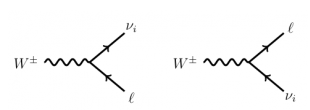
\includegraphics[width=0.6\textwidth]{W_boson.png}
\caption{Všeobecný rozpad W bozónu na leptonový pár.}
\label{sf1:fig:W_boson}
\end{figure}
\newline
Porovnaním predošlej teórie s touto dostávame, že platí
\begin{equation}
\frac{g^2}{8M_W^2}=\frac{G_F}{\sqrt{2}}.
\end{equation}
Keďže, W bozóny sú nositeľmi elektrického náboja tak je s nimi možná aj elektromagnetická interakcia. Postup odvodenia interakcie W bozónu s fotónom si opíšeme len slovne.

Keďže W bozón je hmotná vektorová častica tak musí spĺňať správanie popísane Procovým lagrangianom. V tomto lagrangiane transformujeme polia a derivácie pomocou lokálnej kalibračnej transformácie presne tak isto ako v prípade elektromagnetickej interakcie. Keď sa obmedzíme na členy, ktorých dimenzia nebude vyššia ako 4 tak po par úpravách dostaneme, že interakčný lagrangian medzi W a fotónom ma tvar $\mathcal{L}^{em}=\mathcal{L}_{WW\gamma}+\mathcal{L}_{WW\gamma \gamma}$. Takže náš celkový interakčný lagrangian ma tvar
$$
\mathcal{L}^{ew}=\mathcal{L}^{w}+\mathcal{L}^{em} =\mathcal{L}_{CC}+\mathcal{L}^{em}_{fermion}+\mathcal{L}_{WW\gamma}+\mathcal{L}_{WW\gamma\gamma}.
$$
Aj keď bol tento model navrhnutý, aby sa zbavil predošlých divergencii z Fermiho modelu, pri spojení elektrickej a slabej interakcie nám vznikli procesy, v ktorých sa objavujú ďalšie divergentne členy.
 
Veľký progres vo vývoji prišiel, keď sa aplikovali poznatky plynúce zo štúdie Yang-Millsovej teórie, ktorá je založená na ne-Abelovskej kalibračnej symetrii. Ukázalo sa, že tato symetria môže zrušiť nejaké nežiaduce divergencie. Dôkladné odvodenie perturbatívnej renormalizácie, ktoré je založená na ne-Abeliovskej kalibračnej symetrii a ktoré navyše zahŕňa Higgsov mechanizmus pre generovanie hmoty, bolo odvodene Hooft-om v roku 1971. Rozhodujúcim momentom bol experimentálny objav slabého neutrálneho prúdu v roku 1973, ktorý jasne ukázal, že kalibračný model, ktorý zahŕňa neutrálny vektorový bozón, môže byť použitý na opis reálneho sveta. Tento model bol následne vylepšovaný až nakoniec dospel do tvaru, ktorý navrhli Weinberg, Salam a Glashow, zvaný ako štandardný model elektroslabej interakcie.

Tento model je založený na ne-Abelovskej SU(2) $\times$ U(1) kalibračnej grupe. Príslušnými kalibračnými bozónmy sú 3 W bozóny izospinu z SU(2) grupy ($W_1$, $W_2$, $W_3$) a B bozón slabého-náboja z U(1) grupy. Všetky tieto polia sú bezhmotné. Až ich vzájomná kombinácia bude dávať už nám známe $W^{\pm}, Z^0, \gamma$ bozóny. Hmotnosť týchto častíc (okrem $\gamma$), vyplíva zo spontánneho narušenia symetrie, ktoré je základom tkz. Higgsovho mechanizmu, ktorý je založený na existencii jednej skalárnej, neutrálnej častici so spinom rovný nule - Higgsov bozón. Výsledný lagrangian bude vo všeobecnom tvare následovný
\begin{equation}
\mathcal{L}_{ew}=\mathcal{L}_{K}+\mathcal{L}_{N}+\mathcal{L}_{C}+\mathcal{L}_{H}+\mathcal{L}_{HV}+\mathcal{L}_{WWV}+\mathcal{L}_{WWVV}+\mathcal{L}_{Y},
\end{equation}
kde $\mathcal{L}_{K}$ je kinetický člen pozostavajúci z kvadratických členov, ktoré zahŕňajú dynamické členy a hmotnostných členov, $\mathcal{L}_{N}$ a $\mathcal{L}_{C}$ sú členy, ktoré obsahujú neutrálny a nabitý prúd. Ich komponenty obsahujú interakcie medzi fermiónmy a bozónmy, $\mathcal{L}_{H}$ obsahuje interakčné Higgs three-point and Higgs four-point self interakcie, $\mathcal{L}_{HV}$ obsahuje interakcie Higgsa s W,Z bozónom, $\mathcal{L}_{WWV}$
obsahuje three-point self interakciu W,Z,$\gamma$ bozónov, $\mathcal{L}_{WWVV}$ obsahuje four-point self interakciu W,Z,$\gamma$ bozónov a $\mathcal{L}_{Y}$ obsahuje Yukawovsku interakciu medzi fermiónmy a Higgsových bozónom.

Povedzme si teraz nejaké vlastnosti a výsledky z daného lagrangianu. \textbf{Unification condition} - je vzťah, ktorý viaže väzbové konštanty slabej interakcie a elektromagnetizmu. Táto podmienka môže byť vyjadrená nasledovne 
$$
e=g\sin(\theta_W)=g^,\cos(\theta_W),
$$
kde $q$ je väzbová konštanta pre SU(2) grupu, $q^,$ je väzbová konštanta pre U(1) grupu a $\theta_W$ sa vola weak mixing uhol alebo Weinbergov uhol, ktorým spontánne narušenie symetrie rotuje pôvodne $W_3$ a $B$ vektorové kalibračné bozóny. Experimentálna hodnota tohto uhlu je $\sin^2(\theta_W)=0.222\pm0.006$. Využitím tohto uhla sa dajú dané kalibračné polia nakombinovať tak, že vzniknú $Z^0$ a $\gamma$ bozóny. Graficky sa celá unification condition dá znázorniť nasledovne, viď obrázok \ref{sf1:fig:unifi}.
\begin{figure}[!h]
\centering
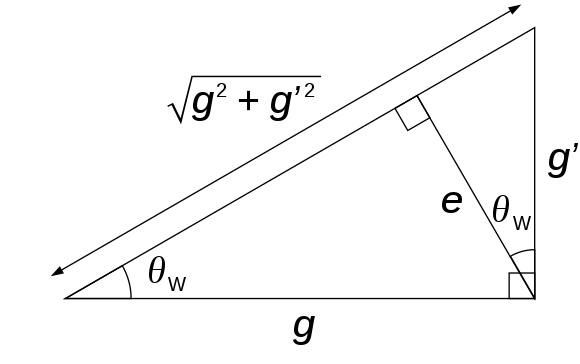
\includegraphics[width=0.6\textwidth]{Unification_condition.png}
\caption{g-väzbová konštanta pre SU(2) grupu, $q^{,}$ je väzbová konštanta pre U(1) grupu.}
\label{sf1:fig:unifi}
\end{figure}

Hmotnosti $W^{\pm}$ a $Z^0$ sa dajú vyjadriť ako 
$$
m_W=\bigg(\sqrt{\frac{\pi \alpha}{G_F\sqrt{2}}}\bigg)\frac{1}{\sin(\theta_W)}=80,42\,GeV/c^2, \hspace{0.5cm} m_Z=\frac{m_W}{cos(\theta_W)}=91.18\,GeV/c^2
$$
Uveďme základne pravidla pre konštrukciu vertexov pre slabé interakcie. V každom vertexe musí byť zachovaný elektrický náboj, leptonové číslo a počet kvarkov. Keďže nabité $W^{\pm}$ bozóny menia náboj kvarku, v slabých vertexoch sa nezachovávajú vône kvarkov. Ich farebný náboj sa ale zachovaná, lebo W bozóny nie sú nositeľmi farebného náboja. Je potrebne tiež zmieniť, že slabé interakcie pôsobiace prostredníctvom W bozónov nemenia generáciu leptónov. Slabé interakcie zahrňujúce W bozón sa nazývajú interakcie nabitých prúdov, naopak slabé interakcie sprostredkúvané Z bozónom sa nazývaju interakcie neutrálnych prúdov. Pravidlá pre vertexy Zqq sú veľmi jednoduché - nemení sa v nich leptónová generácia, kvarková vôňa ani farebný náboj.

\textbf{Miešanie kvarkov, Cabbibov uhol, CKM matice}
Ako sme už spomínali pri odvodzovaní lagrangianu, v 60. rokoch minulého storočia sa ukázali experimenty kedy došlo k tomu, že sa nezachovávala podivnosť. Tie sú síce potlačené oproti tým, čo nemenia podivnosť ale aj tak existujú a to bolo treba vysvetliť a popísať. S popisom prišiel Gabibbo, ktorý si všimol pozoruhodné súvislosti medzi známymi slabými procesmi. Pre procesy, kde sa podivnosť nemení ma efektívna hadrónová konštanta hodnotu $G_F\cos(\theta_C)$, pre podivnosť meniace procesy má táto efektívna konštanta hodnotu $G_F\sin(\theta_C)$. Experimentálne sa určilo, že Gabibbov uhol ma hodnotu $\theta_C=13.04^{\circ}$. V rámci dvoj-generačného modelu (u, s, d, c kvarky) je možné také zmiešavanie popísať pomocou reálnych koeficientov, ktoré je možne súhrnne zapísať do tvaru matice
\[ U_C=
\begin{pmatrix}
    \cos(\theta_C) & \sin(\theta_C) \\
    -\sin(\theta_C) & \cos(\theta_C) \\
\end{pmatrix}=
\begin{pmatrix}
    U_{ud} & U_{us} \\
    U_{cd} & U_{cs} \\
\end{pmatrix}
\]
tato matica popisuje zmiešavanie kvarkov. Toto zmiešavanie sa dá napísať nasledovne 
\[
\begin{pmatrix}
    \bar{u},\bar{c} \\
\end{pmatrix}=
\begin{pmatrix}
    \cos(\theta_C) & \sin(\theta_C) \\
    -\sin(\theta_C) & \cos(\theta_C) \\
\end{pmatrix}
\begin{pmatrix}
    d \\
    s \\
\end{pmatrix}
\]
Pre tri generácie je zmiešavanie kvarkov vyjadrené pomocou Cabibbo-Kobayashi-Maskawovou maticou
\[ V_{CKM}=
\begin{pmatrix}
    V_{ud} & V_{us} & V_{ub} \\
    V_{cd} & V_{cs} & V_{cb} \\
    V_{td} & V_{ts} & V_{tb} \\
\end{pmatrix}
\]
jej elementy sú obecne komplexne (dajú sa parametrizovať pomocou troch uhlov Gabibbovho typu a jednou fázou). Presne vyjadrenie elementov CKM matice patri k hlavným a aktuálnym cieľom experimentálnej časticovej fyziky lebo predstavuje jeden zo zásadných testov správnosti Štandardného modelu elektroslabej interakcie.
\[
\begin{pmatrix}
    \bar{u} & \bar{c} & \bar{t} \\
\end{pmatrix} 
\begin{pmatrix}
    0.975 & 0.221 & 0.022 \\
    0.221 & 0.974 & 0.040 \\
    0.009 & 0.039 & 0.999 \\
\end{pmatrix}
\begin{pmatrix}
    d \\
    s \\
    b \\
\end{pmatrix}
\]
Hodnoty CKM matice na diagonále sú skoro rovnaké veľké a blízko jednotky, čo implikuje napríklad, že $t$ kvark sa s najväčšou pravdepodobnosťou rozpadne na $b$ kvark. Nediagonálne prvky sú zase dosť malé. Obecne platí, že kvark s nábojom $+2/3$ (u, c, t) sa transformuje na kvark s nábojom $-1/3$ (d, s, b) a naopak prostredníctvom nabitého $W^{\pm}$ bozónu, ktorý mení náboj o jednotku. Tiež platí, že sa kvarky rozpadajú v postupnosti od najviac hmotných po tie najmenej hmotne 
$$
t\rightarrow b\rightarrow s\rightarrow u \leftrightarrow d
$$
Nasledujúci obrázok graficky znázorňuje prechody medzi kvarkmi \ref{sf1:fig:Kvarky_prechody}
\begin{figure}[!h]
\centering
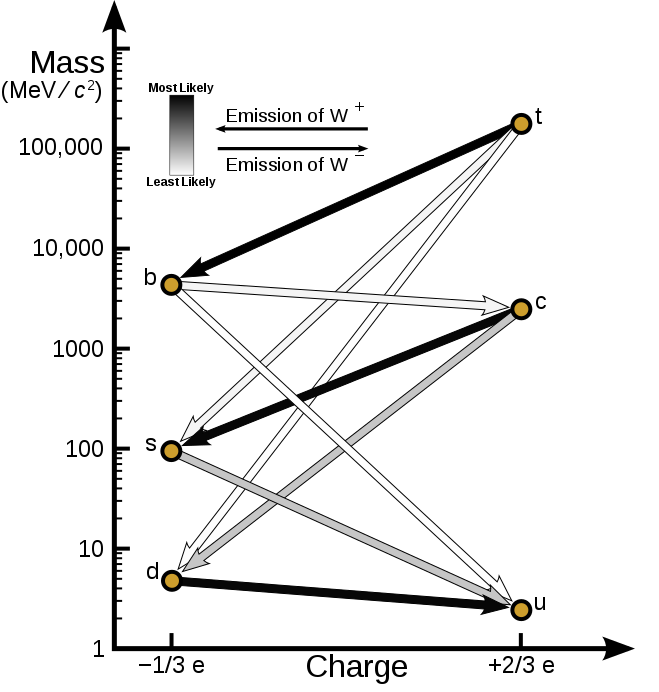
\includegraphics[width=0.6\textwidth]{Kvarky_prechody.png}
\caption{Diagram znázorňujúci prechodové možnosti medzi kvarkmi prostredníctvom slabej interakcie a indikácie pravdepodobnosti prechodov, ktoré sú dane CKM maticou.}
\caption{}
\label{sf1:fig:Kvarky_prechody}
\end{figure}

\subsection{Silná interakcia}
Silná interakcia je sila pôsobiaca len medzi časticami s nenulovým \textcolor{red}{fa}\textcolor{green}{reb}\textcolor{blue}{ným} nábojom. Tento druh náboju obsahujú iba kvarky a preto táto interakcia nie je univerzálna. Táto interakcia je pôsobí len na malých vzdialenostiach medzi hadrónmi a jej dosah je približne $10^{-15}\,m$. Jej prejavmi sú 
\begin{itemize}
	\item jadrové sily medzi nukleónmi v jadre  
	\item sily, ktoré držia kvarky pohromade v nukleóne
	\item produkcia častíc pri vysokoenergetických zrážkach hadrónov
\end{itemize}
Okrem toho, že silná interakcia nie je univerzálna, čiže platí len pre kvarky, tak je aj obmedzená väčším počtom zákonov zachovania ako ostatne interakcie.

Silnej interakcii prislúcha väzbová konštanta, ktorá charakterizuje jej veľkosť
$$
\alpha_s= \frac{g_s^2}{4\pi},
$$
kde $g_s$ je náboj konštituentného kvarku. Pre malé energie je hodnota tejto konštanty $\alpha\approx 1$. Väzbová konštanta pre silnú interakciu je oveľa väčšia ako pre elektromagnetickú interakciu. Veľkosť tejto konštanty pre malé energie ma za následok nepoužiteľnosť poruchovej teórie kvôli divergentným členom. Avšak táto konštanta ma tu vlastnosť, že jej veľkosť závisí od prenesenej energie (resp. hybnosti), preto sa tato konštanta nazýva aj $bežiaca$ väzbová konštanta. S rastúcou energiou interakcie (s rastúcou hybnosťou zrážajúcich sa častíc) totiž táto väzbová konštanta klesá, čo vedie k asymptotickej voľnosti (divergentne členy začnú konvergovať, čo umožni použiť poruchovú teóriu). Závislosť $\alpha_s$ na hybnosti je nasledujúca
$$
\alpha_s\approx\frac{12\pi}{(11n_c-2n_f)\ln\big(\frac{k^2}{\Lambda^2}\big)}
$$ 
kde $n_c$ je počet farebných nábojov, $n_f$ je počet kvarkových druhov častice (flavour) a $\Lambda$ je škálovací parameter vychádzajúci z renormalizačného procesu a má hodnotu približne $200\,MeV$. (Napr. $\alpha_s=0.12$ pre $k^2=(100\,GeV)^2$.)

Mediátorom silnej interakcie je vektorová častica gluón, ktorá je neutrálna a nehmotná, niečo ako fotón pre QED. Avšak, pre elektromagnetickú interakciu máme len dva typy elektrického náboja: kladný a záporný. V teórii silnej interakcie, ktorá je popísaná kvantovou chromodynamikou (QCD), však existuje 6 druhov náboja, ktorý sa z nevysvetliteľnej príčiny nazýva \textcolor{red}{fa}\textcolor{green}{reb}\textcolor{blue}{ný} náboj a sú to tieto, viď obrázok \ref{sf1:fig:Color_quarks}
\begin{figure}[!h]
\centering
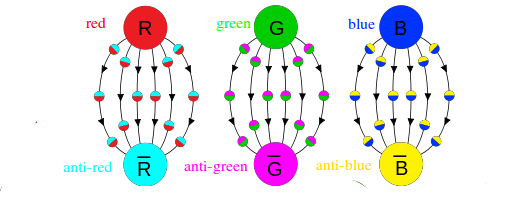
\includegraphics[width=0.6\textwidth]{Color_quarks.png}
\caption{6 druhov kvarkov, horne tri sú farebné náboje red, green, blue a spodné sú ich anti-farebné náboje anti-red, anti-green, anti-blue.}
\label{sf1:fig:Color_quarks}
\end{figure}
\newline
Podľa QCD sú baryóny (častice tvorené z 3 kvarkov) a mezóny (častice tvorené jedným kvarkom a anti-kvarkom) farebne neutrálne. Pre gluóny platí, že sú nositeľmi aj jednej farby aj jednej anti-farby súčasne, kebyže to tak nie tak by potom hadróny nemohli byt viazané vo farebne neutrálnom systéme.  Z toho potom máme celkovo $3^2=9$ možných farebných kombinácii pre gluóny. Avšak, ako vieme, nie je to úplne pravda, že ich je 9. V skutočnosti máme len 8 gluónov a to z toho dôvodu, že bezfarebný singletný stav $\frac{1}{\sqrt{3}}(r\bar{r}+b\bar{b}+q\bar{q})$, nebol zatiaľ experimentálne pozorovaný. Ak by totiž tento singletný stav existoval bolo by možné pozorovať silnú interakciu na väčších vzdialenostiach. Poďme si načrtnúť ako to v takom bezfarebnom systéme vlastne funguje. Majme nasledujúci obrázok \ref{sf1:fig:Prechody}
\begin{figure}[!h]
\centering
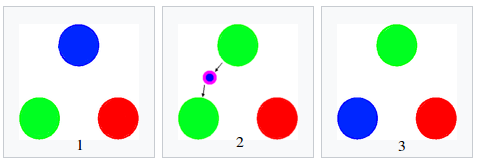
\includegraphics[width=0.8\textwidth]{Color_changing.png}
\caption{}
\label{sf1:fig:Prechody}
\end{figure}
\newline

Na 1. obrázku máme systém, ktorý je bezfarebný a na ktorom zatiaľ neprebieha žiadna výmena gluónu. Na 2. obrázku však už máme gluón, ktorý sa uvoľnil z modrého kvarku. Keďže tento gluón pochádza z modrého kvarku tak jeho farebná polovica musí byť modrá. Ta anti-farebná časť gluónu môže byť prakticky hocijaká. V našom prípade je anti-zelená. Keďže sa odnáša anti-zelená farba tak kvark musí byť zelený aby bol celý systém stále farebne neutrálny. Na 3. obrázku sa gluon absorboval do zeleného kvarku. Tam sa spoločne vybili anti-zelená a zelená farba a jedine, čo z gluónu ostalo je modra farba. Navyše gluóny majú tu vlastnosť, že môžu interagovať medzi sebou, to fotóny napríklad nemôžu. Takže, keď máme systém, kde je viacej gluónov, môže dôjsť k tomu, že gluóny navzájom budú interagovať, čo môže viesť k tomu, že sa zmení ich celkový farebný náboj. Avšak, stále sa nesmie zmeniť celkový farebný náboj systému. Pre názornejšie a krajšie vysvetlenie odporúčam si pozrieť toto video (Introduction to subatomic physics and subatomic particles: Part III na YOUTUBE).

Vzhľadom k tomu, že sú gluóny nehmotné je možne očakávať, že časť statického QCD potenciálu bude podobná QED potenciálu. Tvar efektívneho potenciálu pre ťažké kvarky môže byť aproximovaný nasledujúcim tvarom potenciálu 
$$
V = -\frac{4}{3}\frac{\alpha_s}{r}+kr.
$$ 
Tento potenciál sa nazýva Cornell-ov potenciál a je použiteľný pre systémy ťažkých kvarkov: charmonium a bottomonium. Faktor $4/3$ vyplýva z toho, že máme 8 farebných gluónov, ktoré môžu pôsobiť na 3 kvarky, ktoré majú rôzne farebné náboje. Prvá časť, ktorá je úmerná 1/r, zodpovedá potenciálu vyvolanému výmenou jedného gluónu medzi kvarkom a jeho antikvarkom a je známa ako Coulombická časť potenciálu, pretože jeho forma 1/r je identická s dobre známym Coulombickým potenciálom, ktorý je vyvolaný elektromagnetickou silou. Druhy člen je asociovaný s viazanosťou kvarkov a parametrizuje slabo pochopené non-pertubatívne účinky QCD. Pre veľké vzdialenosti je potenciálna energia medzi kvarkmi tak veľká, že v istom momente sa táto energia premení na novo vzniknutý kvark-antikvark pár. Takže namiesto toho, aby sme dostali oddelený kvark a anti-kvark, dostaneme dva viazané páry kvark-antikvark.

Vertex faktor silnej interakcie pozostáva z kvarkov a gluónov. Základný vertex sa skladá z dvoch fermiónových liniek a jednej bozónovej linky. Ako sme už spomínali vyššie, na rozdiel od QED je možné v tomto prípade mať aj dva vertexy, ktoré zahrňujú troj- a štvor- gluonovú interakciu. Toto je základný rozdiel oproti QED, kde fotóny navzájom medzi sebou neinteragujú. Existencia týchto vertexov v QCD je možná vďaka ne-Abelovskej kalibračnej transformácii. Je to veľmi podobné tomu, čo sme mali pre elektroslabú interakciu. Aj tam sa totiž nachádzajú prípady, kedy dochádza k troj- a štvor- bozónovej interakcii, ktorá je taktiež podmienená touto ne-Abelovskou kalibračnou transformáciou. Akurát tam medzi sebou interagujú $W^{\pm}, Z^0$ a $ \gamma$ bozóny, viď obrázok \ref{sf1:ref:vertexy}.
\begin{figure}[!h]
\centering
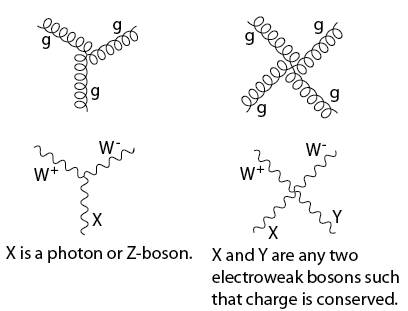
\includegraphics[width=0.5\textwidth]{Vertexy.png}
\caption{}
\label{sf1:ref:vertexy}
\end{figure}
\newline

QCD je typ kvantovej teórie poľa zvanej teória ne-Abelovskej kalibračnej transformácie so skupinou symetrií SU(3), ktorú navrhli páni David Gross, David Politzer a Frank Wilczek. QCD lagrangian má tvar
\begin{equation}
\begin{gathered}
\mathcal{L}_{QCD}=-\frac{1}{4}G^a_{\mu\nu}G^{a\mu\nu}+
\sum_{\psi}\bar{\psi}_i\big(i\gamma^{\mu}(\partial_{\mu}\delta_{ij}-ig_sG_{\mu}^aT_{ij}^a)-m_{\psi}\delta_{ij}\big)\psi_j\\
G_{\mu\nu}=\partial^{\mu}A^{\nu}-\partial^{\nu}A^{\mu}+gf_{abc}A^{\mu}_bA_c^{\nu},
\end{gathered}
\end{equation}
kde $G^{\mu\nu}$ je antisymetrický tenzor, ktorého posledný člen kompenzuje nekomutatívnosť rotácii vo priestore farebného náboja tento posledný člen môže za tú troj- a štvor- gluónovú self-interakciu, $\psi_i$ je Dirakov spinor kvarkového poľa s farebným nábojom i=(r,q,b), $G_{\mu}^a$ je 8 komponentné SU(3) kalibračné pole, $T_{ij}^a$ reprezentuje 3x3 Gell-Mannovú maticu, $g_s$ silná väzbová konštanta.

Existuje veľa spôsobov ako naložiť s QCD. Dá sa k nej pristupovať pomocou poruchovej teórie, ktorá je založená na asymptotickej voľnosti (male $\alpha_s$). Medzi neporuchovými teóriami má najsilnejšie postavenie tkz. Lattice QCD - k redukcii analytických integrabílnych dráhových integrálov sa na numerické výpočty používa sada diskrétnych bodov rozložených na mriežke (lattice). Pre riešenie špecifických problémov sa používajú efektívne teórie, ktoré v istých limitách dávajú kvalitatívne presne výsledky. Takouto teóriou je napríklad chirálna poruchová teória, čo je efektívna teória pre QCD pri nízkych energiách.

\textbf{Hadronizácia} alebo tiež fragmentácia je formovanie hadrónov z kvarkov a gluónov. Tento jav môže nastať po vysoko-energetických zrážkach častíc, kedy sú produkované "voľné" kvarky a gluóny. Takáto produkcia párov môže vzniknúť napríklad anihiláciou pri interakcii $e^-e^+$. Následne medzi kvarkom a antikvarkom nastáva dynamická separácia. Táto separácia nastáva preto lebo novo vzniknuté častice majú veľkú energiu. Existujú dva prístupy ako kvantitatívne pochopiť proces formovania hadrónov: 
\begin{itemize}
	\item Chromostatický prístup \newline
	Kvark-antikvark pár vytvorí ďalší kvark-antikvark pár, akonáhle vzdialenosť medzi kvarkom a anti-kvarkom v páre je rádovo $1\,fm$. Pri takejto vzdialenosti je hustota energie medzi kvarkom a anti-kvarkom natoľko veľká, že dôjde k vytvoreniu ďalšieho páru. Tento proces pokračuje až kým relatívna hybnosť kvarkov neklesne na takú hodnotu, že už nebude môcť dochádzať k tvoreniu ďalších párov, vid obrázok \ref{sf1:fig:anihilation}. Hadróny následne vznikajú pozdĺž reťazca tvorenia kvarkov. Vytvorené hadróny produkujú spŕšku zvanú jety, ktoré sú približne v smere prvého kvarku, respektíve anti-kvarku.
	\begin{figure}[!h]
	\centering
	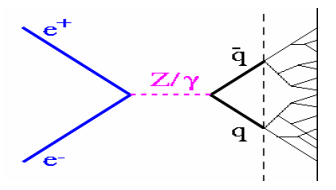
\includegraphics[width=0.3\textwidth]{Anihilation.png}
	\caption{}
	\label{sf1:fig:anihilation}
	\end{figure}
	\item Chromodynamický prístup \newline
	Tento prístup sa odohráva tkz. kvark-gluonovou kaskádou, viď obrázok \ref{sf1:fig:cascade}. Táto kaskáda začína emisiou gluónu kvarkom alebo anti-kvarkom. Tento gluón môže produkovať buď kvark-antikvark pár alebo gluonový pár. Keďže existuje viacej gluónov ako kvarkov tak štatisticky sa tento gluon bude rozpadať viacej na gluóny ako na kvarky. Silná väzba bude narastať so zmenšujúcou sa hodnotou hybnosti virtuálnej častice. Na konci kaskády, kvarky vytvoria bezfarebné viazané stavy. Je jasne, že tento model nemôže byť použitý až na koniec hadronizačného procesu. Dôvodom je, že pre male hodnoty hybnosti sa väzbová konštanta zväčšuje a tým sa narúša poruchový rozvoj. V tejto oblasti prevláda elastický efekt, ktorý skončí tvorbou hadrónov. Hadróny sú tvorené vo vákuu na konci kvark-gluonovej kaskády. Transverzálna hybnosť hadrónov vzhľadom na pôvodný smer kvarku je je limitovaná Heisenbergovým princípom neurčitosti. Hadróny sú preto koncentrované okolo pôvodného smeru kvarku a tvoria jety. Ak ma prvý gluón dostatočne veľkú transverzálnu hybnosť, tak môže vzniknúť tretí hadronový jet v smere tohto gluónu.
	\begin{figure}[!h]
	\centering
	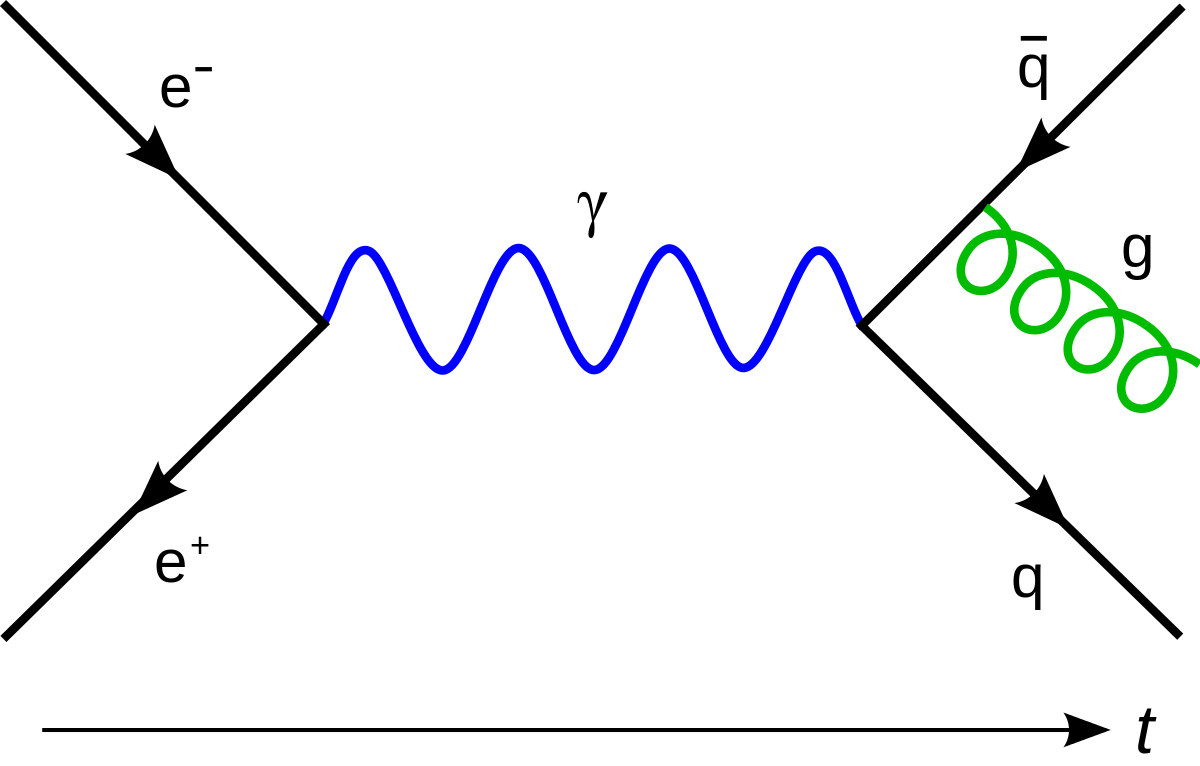
\includegraphics[width=0.3\textwidth]{Cascade.png}
	\caption{}
	\label{sf1:fig:cascade}
	\end{figure}
\end{itemize}

Dynamika týchto hadronizačných procesov stále nie je úplne pochopená pomocou QCD a to vďaka tomu, že poruchová teória v QCD, formulovaná pomocou kvarkov a gluónov, je platná len na malých vzdialenostiach. Na väčších vzdialenostiach sa táto poruchová teória zrúti. Existujú však rôzne fenomenologické modely, ktoré sa to snažia popísať. Prvým takýmto modelom bol Feynmanov a Fieldov, nezávisle vytvorený, fragmentačný model. Základnou myšlienkou tohto modelu je predstava hadronizácie kvark-dikvarkového systému ako nezávislej fragmentácie kvarku a dikvarku. Tento predpoklad je ale v princípe neudržateľný, pretože k hadronizácii dochádza vďaka vzájomnej interakcii medzi nimi. Avšak, ukázalo sa, že výsledné rozdelenie hadrónov môže byť v istom priblížení popísane fragmentačnou funkciou $D^h_q(k,p_T)$ (jazyk fragmentačneho modelu). Ta popisuje pravdepodobnosť, že parton $q$ vytvorí hadrón $h$ nesúci časť $k$ z pôvodnej energie partónu a priečnou hybnosťou $p_T$. Táto funkcia ako každá iná distribučná funkcia by mala byt univerzálna t.j. nezávislá na procese.

\textbf{Jet} je spŕška častíc, ktorá sa nachádza v úzkom kuželi, ktorá vznika pri hadronizácii kvarkov a gluónov. Sú to vlastne experimentálne znaky kvarkov a gluónov produkovaných vo vysoko-energetickej fyzike, viď obrázok \ref{sf1:fig:jet}. 
\begin{figure}[!h]
\centering
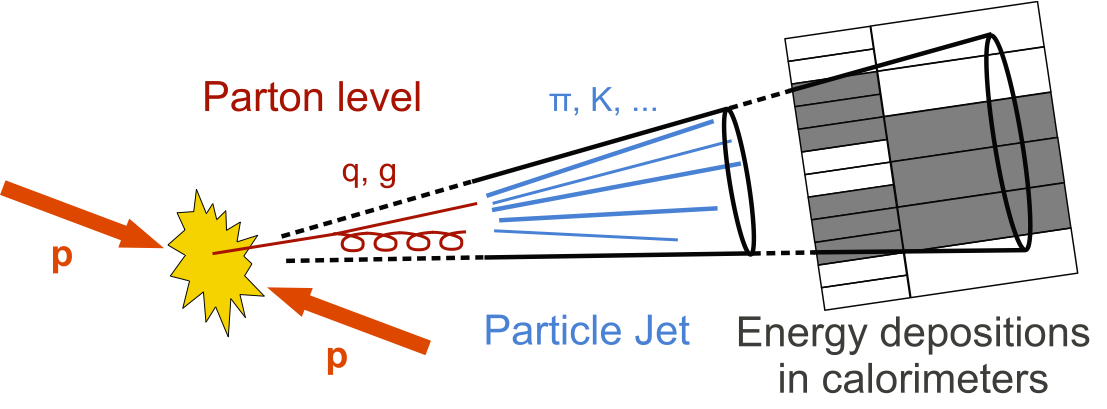
\includegraphics[width=0.7\textwidth]{Jet.png}
\caption{}
\label{sf1:fig:jet}
\end{figure}
Skutočnosť, že smery a energie jetov dobre odpovedajú smerom a energiám pôvodných kvarkov, nie je triviálna vlastnosť procesu hadronizácie. Smerové rozdelenie jetov v priestore vzhľadom k smeru $e^-e^+$ zrážky by malo byt rovnaké ako koncový stav pri procese $e^-e^+\rightarrow \mu^-\mu^+$, pretože mióny a kvarky majú spin 1/2. Tento fakt je jedným zo silnejších dôkazov toho, že kvarky majú spin 1/2. Kvark, anti-kvark a gluon môžu fragmentovať do hadrónov, čo vedie k troj-jetovým eventom. Vzhľadom k tomu, že uhlové rozdelenie jetov je v súlade s teoretickou predpoveďou pre gluón so spinom 1, poskytli tieto eventy jednoznačný dôkaz o existencii gluónov.

\subsection{Gravitačná interakcia}
Táto sila sa uplatňuje len pri silovom pôsobení medzi makroskopickými objektmi a v kozmickej mechanike. V subatómovej fyzike nehrá podstatnú rolu a preto môže byť zanedbaná. Staršia teória gravitácie pochádza od Newtona, ktorý túto silu popísal ako $$ \vec{F}=\kappa\frac{m_1m_2}{r^2}\frac{\vec{r}}{r}, $$ kde $\kappa=6.672\times10^-11\,m^3kg^-1s^2$, je väzbová konštanta. Jej pôsobenie je nekonečné, podobne ako pre elektromagnetickú interakciu. Dá sa povedať, že to je najdemokratickejšia sila akú poznáme. Pretože je univerzálna. Modernou teóriou gravitácie je Všeobecná teória relativity, ktorá tvrdi, že zrýchlenie a gravitačná sila je ta istá vec. Sprostredkovateľom tejto interakcie je gravitón (zatiaľ nebol pozorovaný), ktorý by mal byt nehmotný a mal by mat spin rovný 2.

\section{Vlastnosti leptónov a hadrónov}
Sem si pripomenieme vlastnosti, ktoré sme hore neuviedli. A ak spomeniem niečo, čo sa bude opakovať tak je dôležité a je dobre si to znovu pripomenúť.\newline
\textbf{Leptóny}
\begin{itemize}

\item Leptóny nemajú farebný náboj a tak nepodliehajú silnej interakcii podobne ako neutrína, ktoré nemajú elektrický náboj a tak nepodliehajú elektromagnetickej interakcii. Neutrína interagujú jedine slabou interakciou.
\item Keďže leptóny majú nenulový spin, môžu vytvárať magnetické pole. Veľkosť magnetického dipolového momentu je daný 
$$\mu=g\frac{Q\hbar}{4m},$$ kde $m$ je hmotnosť leptónu, $g$ je tkz. g-faktor pre leptón. Prvý rad približnej kvantovej mechaniky predpovedá túto hodnotu rovnú 2 pre všetky leptóny. Avšak, vyššie rady kvantového efektu spôsobujú korekciu tejto hodnoty označovanú ako anomálny magneticky moment. Toto číslo je veľmi citlivé na veľa detailov a preto jeho spočítanie a následne experimentálne zmeranie bolo obrovským úspechom QED. Vo Feynmanových diagramoch toto číslo reprezentujú slučky. Tato korekcia má približne hodnotu $a_e=0.001159....$ 
\item Všetky leptóny, okrem tau neutrína, boli pozorované priamo v experimentoch - ako voľné častice.
\item Presne merania miónových vlastnosti boli vykonané prostredníctvom skúmania mezoatómov vytvorených zachytením miónu v atóme na Bohrovej orbite. Hodnota energie stavu mezoatómu s hlavným kvantovým číslom $n$ je lineárne úmerná hmotnosti miónu $$E(n)=-\frac{Z^2e^4m}{2(4\pi\epsilon_0)^2\hbar^2n^2}$$ a teda je v absolútnej hodnote asi 200-krát väčšia než energie odpovedajúce tomu istému stavu ale s elektrónom. Prechod do stavu z nižšou hladinou energie spôsobuje emisiu röntgenového žiarenia, ktoré je charakteristické a možno z neho vyvodiť informácie o náboji, hmotnosti a spine.
\item Doba života miónov je okolo $\tau_0=2.2\mu s$ a ich rýchlosť je $\beta=0.98$. Veľká časť miónov vzniká vysoko v atmosfére, asi $10\,km$ nad zemou. Keďže sa tieto mióny pohybujú tak rýchlo nastáva dilatácia času vzhľadom na pozorovateľa na Zemi. To znamená, že vo svojej sústave má mión dobu života tých $\tau_0$ ale v sústave pozorovateľa, ktorý stoji na zemskom povrchu a sleduje mióny je ten čas o čosi dlhší, presnejšie $\tau=\tau_0/\sqrt{1-\beta^2}\approx11\mu s$. Takže dráhu, ktorú prejde mión určime veľmi jednoducho  $l=\beta c\tau \approx 13.2\,km$. A preto je možné, že pozorujeme kozmické mióny na povrchu Zeme. Toto je aj jeden z dôkazov Špeciálnej teórie relativity.
\item Dominantný rozpad miónu: $\mu^-=e^-+\bar{\nu}_{e^-}+\nu_{{\mu}^-}$. Ostatne možné rozpady napr. $\mu^-=e^-+\gamma$ je síce kinematický možný ale nezachováva sa flavor číslo. Takéto rozpady majú $BR\sim10^{-12}$.
\item Helicita častice je vyjadrenie orientácie medzi spinom častice a jej hybnosťou. Častice, ktorých spin je orientovaný v rovnakom smere ako hybnosť, sú pravo-točivé a v prípade, že orientácia je v protismere tak hovorime o ľavo-točivých časticiach. Pre QCD a QED sú častice rovnako pravo a ľavo točivé, nedochádza tam k žiadnej asymetrii. Avšak, v prípade slabej interakcie máme len ľavo-točivé fermióny a pravo-točivé neutrína - maximálne narušenie parity.
\item Elektricky náboj môže byť spočítaný z projekcie spinu a slabého-hypernáboja cez $Gell-Mann-Nishijima$ formulu $$Q=T_3+\frac{Y_W}{2}$$.
\item Kinetická energia $\beta$ častica má spojité spektrum od 0 až po maximálne predanú energiu. Typická energia je $1\,MeV$, ale v extrémnych prípadoch to môže byť aj niekoľko $10\,MeV$. Fundamentálny $\beta$ rozpad nastáva vďaka konverzii d-kvarku neutrónu na u-kvark protónu emisiou $W^-$ bozónu, ktorý sa následne rozpadá na $e^-$ a $\nu_{e^-}$.
\item $\Gamma\sim KG_F^2m_l^5$, kde $K$ je číselná konštanta, $G_F$ je Fermiho konštanta a $m_l$ je hmotnosť leptónu. Stredná doba života je $\tau=\hbar/\Gamma$
\item Kvarky, ktoré určujú vlastnosti hadrónov sa nazývajú valenčné kvarky. Hadróny naviac obsahujú tiež prchavé kvark-antikvark páry, ktoré nemenia vlastnosti, ale prispievajú k jeho pokojovej energii. Tieto kvarky sa nazývajú morské kvarky.
\item $$ R=\frac{\sigma(e^+e^-\rightarrow q\bar{q})}{e^+e^-\rightarrow \mu^+ \mu^-}=3\Sigma_{q}e^2_q$$ tento pomer je založený na tom, že existujú tri farebné stavy kvarkov a je na energii takmer nezávislý. Porovnaním experimentálnych dát vychádza, že to sedí.\newline
\end{itemize}
\textbf{Hadróny}
\begin{itemize}
	\item Vlastnosti hadrónov ako náboj, spin, atď. sú určene valenčnými kvarkmi, zatiaľčo hmotnosť hadrónov ma s valenčnými kvarkmi veľmi malo spoločné a veľká časť hmotnosti pochádza z množstva energie, ktorú prenášajú gluóny.
	\item Hadróny sa rýchlo rozpadajú silnou interakciou, pokiaľ im to umožnia kvantové čísla (zákony zachovania kvantových čísiel). Ďalej potom už pracuje slabá interakcia, ktorá mení vôňu kvarkov až na kvarky prvej generácie a nakoniec až na nejaké leptóny.
	\item Najťažšie známe častice, vznikajúce pri časticových interakciách pri vysokých energiách, sú hadróny zvané hyperóny. Všetky hyperóny vykazujú silnú interakciu a sú vysoko nestabilné s veľmi krátkou dobou života. Vzhľadom k tomu, že hyperóny interagujú silnou interakciou, môžu vstupovať do jadier a byť tam naviazané jadrovými silami - vzniknú hyperjadrá. V typickom hyperjadre je jeden nukleón nahradení hyperónom. Sú to nestabilne útvary, ktoré sa rozpadajú dvojako: buď mezónovým rozpadom alebo nukleónovým rozpadom.
	\item Hypernáboj je definovaný ako $Y=B+S+C+T+\tilde{B}$, kde jednotlivé znaky sú baryonóve číslo, podivnosť, pôvab, topness a beauty - kvantové čísla. Následne vďaka tomu môžme spočítať priemet izospinu $I_3=Q-Y/2$, kde $Q$ je elektricky náboj.
\end{itemize}

\section{Symetrie a zákony zachovania}
\textbf{Izospin}\par
Fyzikálna veličina, ktorú zaviedol v roku 1935 Eugene Paul Wigner, aby mohol popísať multiplety rôznych častíc. Jedná sa o kvantové číslo súvisiace so silnou interakciou. Častice, na ktoré pôsobí silná interakcia rovnako, ale ktoré majú rôzny elektrický náboj, môžme považovať za jedinú časticu s hodnotou izospinu súvisiacou s počtom nabitých stavov. Izospin je bezrozmerná veličina a jej názov je odvodený od skutočnosti, že matematické štruktúry, ktoré popisuje, sú podobné tým, ktoré popisuje vnútorný moment hybnosti, zvaný spin.

Niektoré častice majú mnoho spoločných znakov, preto je možné ich chápať ako obmeny jediného objektu. K rozlíšeniu týchto stavov sa zavádzajú rôzne kvantové čísla, z ktorých najčastejším je izospin. Také skupiny príbuzných elementárnych častíc sa nazývajú multiplety. Častice v multiplete sa vzájomne líšia projekciou izospinu. Všetky častice multipletu majú rovnakú veľkosť izospinu a líšia sa projekciou izospinu do ľubovoľnej osy, viď obrázok \ref{sf1:fig:Baryon_decuplet}.\par
\begin{figure}[!h]
\centering
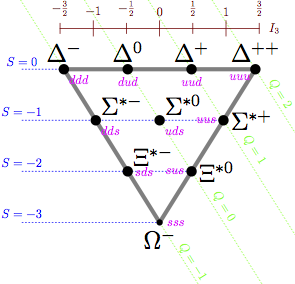
\includegraphics[width=0.5\textwidth]{Baryon_decuplet.png}
\caption{Kombinácia troch u, d alebo s-kvarkov tvoriacich baryóny so spinom 3/2 tvorí baryónový decuplet.}
\label{sf1:fig:Baryon_decuplet}
\end{figure}
Častice v rámci jedného multipletu sa od sebe odlišujú prevážne elektrickým nábojom, popísaným zetovou zložkou izospinu. Naopak príbuzné častice v multiplete majú rovnakú hodnotu spinu, baryónového čísla a podobnú pokojovú hmotnosť. Zistilo sa, že pri procesoch spôsobovaných silnou interakciou sa hodnota izospinu zachováva, zatiaľčo v procesoch elektromagnetickej interakcie sa hodnota izospinu môže zvýšiť alebo znížiť o jednotku.

Počet častíc v multipletoch je daný hodnotou izospinu. Napríklad pre nukleón je hodnota izospinu 1/2, multiplet má teda dve častice neutrón a protón a nazývame ho izospinovým dubletom. Ak je hodnota izospinu 1, má multiplet 3 častice, príkladom môže byť kladný, záporný a neutrálny pión, takýto multiplet nazývame triplet. Existujú tiež singlety, pre ne je izospin rovný 0. Príbuzné častice v multiplete, napríklad protón a neutrón, môžme považovať za rôzne kvantové stavy jednej častice = nukleón. Izospin tieto častice odlišuje.\newline
\textbf{Ďalšie hadrónové čísla}\par
Popri izospinu ešte máme tieto kvantové čísla, ktoré sú charakteristické len pre hadróny. Sú to baryónové číslo B, podivnosť S, pôvab C, beauty B, topness T. 

Obrázok \ref{sf1:fig:zzachovania} znázorňuje veličiny a ich zachovávanie sa v rôznych interakciách. 
\begin{figure}[!h]
\centering
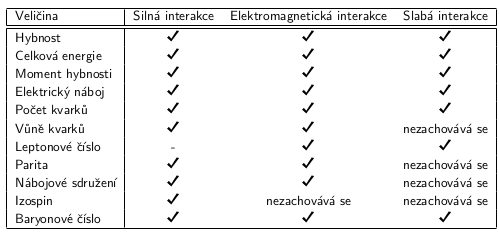
\includegraphics[width=0.9\textwidth]{Zakony_zachovania.png}
\caption{Tu len pripomeniem, že baryónové číslo je definovane ako $B=\frac{1}{3}(n_q+n_{\bar{q}})$. Pre leptónové číslo platí $L=n_l-n_{\bar{l}}$, tu musí byť zachovaný aj flavor leptónu. Napríklad takýto proces nie je pozorovaný: $\mu^- \rightarrow e^-+\gamma$.}
\label{sf1:fig:zzachovania}
\end{figure}
\newline
Skôr ako prejdeme ku samotným zákonom, vysvetlíme najprv význam zákonu zachovania. So zákonmi zachovania veľmi súvisia transformácie. Predpokladajme, že máme systém popísaný ľubovoľnými súradnicami, napr. $\vec{r}=x,y,z.$ Následne posunieme systém po osi $x$ o vzdialenosť $a$. Prepokladajme, že fyzikálny popis systému sa týmto nezmení, tzn. chovanie systému je invariantné voči posunutiu pozdĺž osi $x$.

V teoretickej fyzike existuje teorém, ktorý spojuje invarianciu vzhľadom k danej transformácii so zachovávajúcou sa veličinou-\textbf{Noetherovej teorém}: Každej grupe transformácii súradníc závislých spojito na reálnom parametri, pri ktorých Lagrangeova funkcia zostáva invariantná, odpovedá prvý integrál Lagrangeových rovníc tejto sústavy $=$ zákon zachovania. V našom prípade, invariancia vzhľadom k posunutiu v $x$-ovej osi, sa teda dostaneme k zachovaniu $x$-ovej zložky hybnosti. Táto invariancia sa nazýva symetria systému.
 
Uvedieme zhrnutie týchto spojitých transformácii,  viď obrázok \ref{sf1:fig:zzachovania}, a k ním pridružíme zachovávajúce sa veličiny za predpokladu, že systém je invariantný voči daným transformáciám
\begin{figure}[!h]
\centering
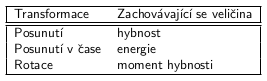
\includegraphics[width=0.5\textwidth]{spojite_trans.png}
\caption{Spojite transformácie a s nimi spojené zachovávajúce sa veličiny. Všetky spojité transformácie sú spojené s aditívnymi kvantovými číslami. Aditívne v tom zmysle, že všetky príspevky rôznych časti systému sa sčítajú do celkovej hodnoty.}
\label{sf1:fig:spojtran}
\end{figure}
\newline
Spojite transformácie majú tú vlastnosť, že každá transformácia môže byť vyjadrená ako súčet malých transformácii. Opakom k týmto transformáciám sú transformácie diskrétne, ktoré nemôžu byť vyjadrené pomocou menších transformácii. Medzi diskrétne veličiny patrí Parita, Nábojové združenie alebo Time reversal.\newline

\textbf{Parita} \par
Pred rokom 1956 fyzici verili, že zrkadlový obraz akéhokoľvek fyzikálneho procesu reprezentuje ďalší možný fyzikálny proces. A práve v tomto roku bol Lee-om a Yang-om navrhnutý experimentálny test, ktorý mal zistiť či je to pravda, a to aj pri pôsobení slabej interakcie. V tomto experimentu boli poctivo zrovnané spiny jadier $^{60}Co$ tak, aby mierili všetky do jedného smeru (povedzme, že napríklad hore). Kobalt sa následne rozpadol beta rozpadom a bol pozorovaný smer vyletujúcich elektrónov. Tento smer pre podstatnú väčšinu elektrónov bol v smere spinu jadier kobaltu.
 
Toto jednoduché pozorovanie malo však udivujúce následky. Predpokladajme, že pozorujeme zrkadlový obraz tohto procesu. Obraz jadra rotuje opačným smerom (spin smeruje dolu). Zrkadlové elektróny ale aj tak vylietavajú smerom hore, ako to bolo v predchádzajúcom prípade. V zrkadlovom odraze sú tak elektróny emitované v smere opačnom k smeru spinu jadier. Mame tak fyzikálny proces, ktorého zrkadlový obraz nepozorujeme v prírode. Parita sa tak pri slabých interakciách nezachováva (pokiaľ by sa zachovávala tak elektróny by boli emitované rovnomerne v oboch smeroch). Nezachovanie parity je stopou slabej interakcie.

Najviac zreteľne je narušenie parity v správaní neutrín. Vieme, že neutrína sú ľavotočivé a anti-neutrína sú pravotočivé. Relatívne jednoduchou nepriamou metódou merania helicity neutrín je využitie rozpadu piónu: $\pi^- \rightarrow \mu^-+\bar{\nu}_{\mu}$. Pokiaľ je pión v kľude, mión a anti-neutríno sú emitované v opačnom smere. Keďže pión má nulový spin, spiny miónu a anti-neutrína musia byt opačne. V prípade, že anti-neutríno je pravotočivé, musí byť aj mión pravotočivý (v kľudovej sústave piónu), čo je overene experimentálne (to že sú oba pravotočivé vychádza z definície helicity-smer spinu je paralelný so smerom hybnosti danej častice).

Navzdory narušenia parity v slabej interakcii, v silných a elektromagnetických interakciách sa parita zachováva. Je teda užitočne vytvoriť formalizmus a terminológiu pre operáciu parity. Označme operator parity ako $\hat{P}$. Pokiaľ tento operator aplikujeme na vektor $\vec{a}$, tak vytvorime vektor do opačného smeru: $\hat{P}\vec{a}=-\vec{a}$. Uvažujeme teraz vektorový súčin $\vec{c}=\vec{a}\times \vec{b}$. Operátor parity zmení znamienko obidvom vektorom, a tak vektorový súčin nezmení znamienko: $\hat{P}\vec{c}=\vec{c}$. Podobná situácia je aj pre skaláry. Operácia parity môže byť zhrnutá nasledovne 
\begin{equation*}
\begin{gathered}
Skalar: \hat{P}s=s  \hspace{2cm} Pseudoskalar: \hat{P}p=-p    \\
Vektor: \hat{P}\vec{v}=-\vec{v}  \hspace{2cm} Pseudovektor: \hat{P}\vec{a}=\vec{a}
\end{gathered}
\end{equation*}
Pri dvojnásobnej aplikácii operátora parity dostaneme pôvodný stav, platí teda $\hat{P}^2=I$, $I$ je jednotková matica. Vlastnými hodnotami tohoto operátora sú $\pm1$.

Majme teraz vlnovú funkciu $\psi(\vec{r})$, ktorá popisuje určitý system. Keď na ňu aplikujeme operator parity dostávame $$ \hat{P}\psi(\vec{r})=\psi(-\vec{r}).$$ Pokiaľ je tato funkcia vlastnou hodnotou tohto operátora, tak podobne ako pre normálny vektor môžme písať
$$ \hat{P}\psi(\vec{r})=\pm \psi(\vec{r}),$$ kde vlastne funkcie operátora $\hat{P}$ s vlastnou hodnotou $(+1)$ nazveme párne (sudé), zatiaľčo tie s vlastnou hodnotou $(-1)$ nazveme nepárne (liché). V prípade centrálnych interakcii, kedy vlnovú funkciu závislú na $\vec{r}$ môžme napísať ako súčin radiálnej vlnovej funkcie a sférickej vlnovej funkcie závislej na orbitálnom momente hybnosti $l$ a jeho projekcii $m$ do z-tovej osy $$ \psi(\vec{r})= R(r)Y_l^m(\theta, \varphi),$$ môžme transformovať $\vec{r}\rightarrow -\vec{r},\theta\rightarrow \pi - \theta,\varphi\rightarrow \pi+\varphi$. Odtiaľto vidíme, že stavy častice pohybujúce sa v poli centrálnych sil s párnym orbitálnym momentom hybnosti $l$ majú párnu paritu a stavy s nepárnym $l$ majú nepárnu paritu.

Mimo parity spojenej s orbitálnym pohybom častice zavadziame aj tkz. $vnútornú$ $paritu,$ ktorá je buď kladná alebo záporná. Veľmi ľahko sa dá pochopiť v prípade hadrónov, ktoré majú vnútornú štruktúru. Avšak, aj elementárne častice majú vnútornú paritu, ktorá je chápaná ako charakteristicky rys danej častice.

Hadróny sú vlastne stavy $\hat{P}$ a je ich možné klasifikovať pomocou vlastnej hodnoty parity, rovnako ako sú klasifikácie pomocou spinu, náboja, izospinu, podivnosti atď. Parita fermiónov musí byť opačná k parite odpovedajúcej antičastice, parita bozónu musí byť musí byť totožná s paritou danej antičastice. Pokiaľ priradíme kvarkom kladnú vnútornú paritu, anti-kvarky ju musia mat zápornú. Parita zloženého systému v základnom stave je produktom (súčinom) parít jeho konštituentov (multiplikatívne kvantové číslo) - preto majú baryóny kladnú paritu a mezóny zápornú. Pre excitované stavy platí $(-1)^l$, kde $l$ je moment hybnosti.

Majme napríklad rozpad $\rho_0 \rightarrow \pi^+ \pi^-$. Vieme, že spin pre $\rho$ je rovný 1 a pióny majú spin rovný 0, preto výsledný piónový stav ma $l=1$. Ďalej vieme, že vnútorná parita $\rho$ mezónu a piónov je (-1). Platí potom $(-1)=(-1)(-1)(-1)^l$, kde v našom prípade $l=1$. Vidíme, že celková parita sa zachováva a nič nebráni aby tento proces nastal.
 
Zoberme si ale teraz prípad $\rho_0 \rightarrow \pi^0 \pi^0$. Tu platí skoro všetko, čo pre predchádzajúci prípad. Nastáva tu však jeden problém. A to taký, že mame dva rovnaké bozóny, ktoré sa musia riadiť Bose-Einsteinovou štatistikou a tak musia vytvoriť symetrickú funkciu. Avšak pre $l=1$ máme iba anti-symetrickú vlnovú funkciu a z toho dôvodu tento proces nemôže nastať.
\newline

\textbf{Nábojové združenie}\par
Vo fyzike elementárnych častíc zavadziame operáciu, ktorú nazývame $nábojové$ $združenie$ $\hat{C}$. Táto operácia konvertuje časticu na jej anti-časticu: $\hat{C}\lvert{p}\rangle=\lvert{\bar{p}}\rangle$.

Názov nábojové združenie je však trochu nevhodný pretože $\hat{C}$ môžme aplikovať aj na neutrálne častice a výsledkom je prevrátená hodnota znamienok u všetkých vnútorných kvantových čísiel, tj. náboj, baryónové číslo, leptónové číslo, podivnosť atď., pričom hmota, energia, hybnosť a spin danej častice zostanú nedotknuté. Rovnako ako u parity aj v tomto prípade, keď zapôsobíme na stav dvakrát dostávame pôvodný stav, tj. $\hat{C}=I$ a vlastnými hodnotami sú tiež $\pm1$. Pre $\lvert p\rangle$, ktoré je vlastným stavom $\hat{C}$, platí $\hat{C}\lvert p\rangle = \pm\vert p \rangle=\lvert\bar{p} \rangle$, kde $\lvert\bar{p} \rangle$ a $\lvert p \rangle$ sa líšia len znamienkom, čo znamená, že reprezentujú ten istý fyzikálny jav. Odtiaľto je zrejme, že len tie častice, ktoré sú svojimi vlastnými anti-časticami, môžu byť vlastnými stavmi $\hat{C}$, čiže sú to fotóny a mezóny ležiace uprostred diagramov Eightfold way.

Systém zahrňujúci častice so spinom $1/2$ a ich anti-častice v konfigurácii s momentom hybnosti $l$ a celkovým spinom $s$ predstavujú vlastný stav $\hat{C}$ s vlastnou hodnotou $(-1)^{l+s}$. Podľa kvarkového modelu tak pre mezóny platí: pseudoskaláry majú $l=0$ a $s=0$, a teda $C=+1$, vektory $l=0$ a $s=1$ majú $C=-1$. $C$ je multiplikatívne kvantové číslo a rovnako ako parita sa zachováva v silných a elektromagnetických interakciách. Preto napríklad $\pi^0 \rightarrow \gamma + \gamma$, kde $C=+1$ pred i po reakcii ale nemôže sa rozpadať na tri fotóny (pre system pre n fotónov je $C=(-1)^n$). Na druhú stranu $C$ sa nezachováva pri slabých interakciách. Pokiaľ by sme $C$ aplikovali na ľavotočivé neutríno, dostali by sme ľavotočivé anti-neutríno, ktoré však neexistuje.\newline

\textbf{Time reversal = Časová inverze}\par
Zmena toku času $t\rightarrow -t$. Prevrátenie toku času tiež prevráti časovú deriváciu priestorových veličín, čo znamená obrátenie všetkých hybnosti $\vec{p} \rightarrow -\vec{p}$ a momentov hybnosti. $\vec{L} \rightarrow -\vec{L}$. Invariancia vzhľadom k tejto transformácii má za následok, že pokiaľ by sme mali dva procesy, z nich druhý by bol opačný k tomu prvému, boli by oba dva rovnako pravdepodobne. Vďaka tejto invariancii tak môžme použiť účinné prierezy atómových alebo jadrových reakcii v oboch smeroch reakcii. Zatiaľ nebol nájdený žiaden dôkaz toho, že to tak nie je. 
\begin{figure}[!h]
\centering
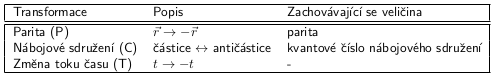
\includegraphics[width=0.8\textwidth]{Diskretnetran.png}
\caption{Diskrétne transformácie a ich vlastnosti.}
\label{sf1:fig:Diskretnetran}
\end{figure}
\newline
\textbf{CP symetria a jej narušenie}\par
Naznačili sme, že slabé interakcie narušujú paritu (P) a aj nábojové združenie (C). Pôvodne sa komunita fyzikov domnievala, že kombinácia CP symetrie zostava slabými interakciami nenarušená. Platilo by totiž $\hat{C}\hat{P}\nu_{L}=\hat{C}\nu_P=\nu_{\bar{P}}$.

K experimentálnemu narušeniu CP symetrie sa dospelo v roku 1964 v BNL objavením anomálii v rozpade neutrálneho kaónu. Bolo totiž zistené, že neutrálne kaóny sa môžu premeniť na svoje anti-častice a naopak ale k týmto prechodom nedochádzalo s presne rovnakou pravdepodobnosťou v oboch smeroch $\rightarrow$ mierne narušenie CP symetrie. Vďaka narušeniu CP invariancie v silnej interakcii prebiehali procesy mierne nesymetrický a viedli k veľmi malému narušeniu rovnováhy medzi hmotou a anti-hmotou. Zhruba na jednu miliardu reakcii oboma smermi prebehlo o jednu reakciu viac smerom k hmote. Keď sa Vesmír dostatočne ochladil došlo k anihilácii latky s anti-latkou. Pri tejto anihilácii však na každú miliardu častíc a anti-častíc zostala kvôli narušeniu CP symetrie jedna častica hmoty. Práve z týchto častíc je dnešný vesmír postavený.

Narušenie CP symetrie bolo pozorované až v roku 2001 na detektore BABAR na Stanforde. Sledovane boli rozpady častice $B^0$ a jej antičastice $\bar{B}^0$. Rozpad oboch častíc môže prebiehať mnohými spôsobmi. V týchto rozpadoch bolo tiež možné sledovať vzácny rozpad na dvojicu pión a kaón, $B^0 \rightarrow K^+ \pi^-$ alebo $\bar{B}^0 \rightarrow K^- \pi^+$.

V prípade rovnakých vlastnosti hmoty a anti-hmoty by obe reakcie mali prebiehať rovnako pravdepodobne a mali by sa objavovať rovnaké počty častíc $K^- \pi^+$ a $K^+ \pi^-$. Skutočnosť ale bola iná. V experimente bolo namerané 910 párov $K^+ \pi^-$ a len  695 $K^- \pi^+$. Spôsob rozpadu hmoty a anti-hmoty tak prebiehal odlišne.

Narušenie CP symetrie je v Štandardnom modely zahrnuté zavedením komplexnej fázy v CKM matici popisujúcej miešanie kvarkov. V tejto schéme je pre komplexnú fázu nevyhnutnou podmienkou existencia najmenej troch generácii kvarkov. Podľa CPT teorému odpovedá narušenie CP symetrie narušeniu invariancie vzhľadom ku zmene toku času. Keby CP bola skutočnou symetriou potom by prírodne zákony platili rovnako ako pre hmotu tak aj pre anti-hmotu.
\newline 
\textbf{CPT teorém}\par
Vo fyzikálnych javoch sa zachováva CPT symetria. Kombinácia všetkých diskrétnych transformácii sa pokladá za nenarušenú vo všetkých fundamentálnych interakciách a zároveň za základnú vlastnosť fyzikálnych zákonov. CPT teória konkrétne prehlasuje, že všetky lokálne interagujúce polia, ktorých lagrangiany sú invariantné vo vlastnej Lorentzovskej transformácii, sú invariantné voči kombinovanej transformácii nábojového združenia, parity a časovej inverzie. Experimentálne preverovanie tejto invariancie sa robilo porovnávaním vlastnosti častíc s ich anti-časticami. Pokiaľ je totiž CPT teorém správny, každá častica musí mať presne rovnakú hmotu a dobu života ako jej odpovedajúca anti-častica. Prebehlo mnoho meraní párov častica-antičastica. Najcitlivejšie overené rozdiely poskytol par $K^0-\bar{K}^0$, viď obrázok \ref{sf1:fig:MeranieCPT}.
\begin{figure}[!h]
\centering
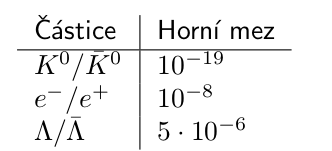
\includegraphics[width=0.3\textwidth]{MeranieCPT.png}
\caption{Relatívne hmotnostne rozdiely medzi časticami a anti-časticami.}
\label{sf1:fig:MeranieCPT}
\end{figure} \newline
Relatívne rozdiely medzi hmotnosťami častíc a anti-častíc sa robilo pomocou $$\delta(m)=\frac{m-\bar{m}}{m+\bar{m}} $$. Zo stredných dôb života miónov bola stanovená horná medza pomerov na $$ \frac{\tau(\mu^+)-\tau(\mu^-)}{\tau(\mu^+)+\tau(\mu^-)}<10^{-4} $$. S veľkou presnosťou boli zmerané magnetické momenty elektrón-pozitrón a mión-antimión. Výsledky sú obvykle prezentované v pojmoch gyromagnetických faktorov $g$, ktorými sú vyjadrené magnetické momenty častíc. Pre elektróny máme $$ \frac{g(e^+)-g(e^-)}{g(e+)+g(e^-)}<10^{-12} $$. Obdobná veličina pre mióny ma hornú medzu $10^{-8}$. Všetky experimentálne dôkazy podporujú invarianciu všetkých interakcii voči transformácii CPT. Pokiaľ je totiž invariancia niektorej z operácii narušená, musí byť kompenzovaná ostatnými transformáciami. Napríklad narušenie invariancie vzhľadom k časovej inverzii, musí byť tiež narušená invariancia vzhľadom k CP.

Dôsledkom CPT symetrie je to, že sa zrkadlový obraz nášho vesmíru, teda otočenie všetkých objektov s ich pozíciami v ľubovolnej rovine (odpovedajúce inverzii parity), obrátenie všetkých hybnosti (odpovedajúce časovej inverzii) a nahradenie všetkej hmoty antihmotou (co odpovedá nábojovej inverzii), bude vyvíjať presne podľa známych fyzikálnych zákonov. CPT transformácia zmení náš vesmír na jeho zrkadlový obraz a naopak.

Dôsledkov platnosti CPT symetrie je hneď niekoľko
\begin{itemize}
	\item Častice s celočíselným spinom podliehajú Bose-Einsteinovej štatistike, zatiaľčo častice s poločíselným spinom podliehajú Fermi-Diracove štatistike.
	\item Častice a ich anti-častice majú totožné hmotnosti a doby života.
	\item Všetky vnútorne čísla častíc sú opačne k vnútorným kvantovým číslam prislúchajúcich antičastíc.
\end{itemize}

\section{Súradnicové sústavy v subjadrovej fyzike}
Transformácie kinematických veličín medzi sústavami, Mandelstamové premenné,\newline
\textbf{Mandelstamové premenné}\par
Mandelstamové premenné sú číselné veličiny, ktoré kódujú energiu, hybnosť a uhly častíc v rozptylovom procese Lorentzovo-invariantným spôsobom. Používajú sa na rozptylové procesy dvoch častíc na dve častice, viď obrázok \ref{sf1:fig:Mandelstam}. V Minkovského metrike diag(1,-1,-1,-1) majú tieto premenne nasledujúci tvar
\begin{equation}
\begin{gathered}
s=(p_1+p_2)^2=(p_3+p_4)^2 \\
t=(p_1-p_3)^2=(p_4-p_2)^2 \\
u=(p_1-p_4)^2=(p_3-p_2)^2
\end{gathered}
\end{equation}
\begin{figure}[!h]
\centering
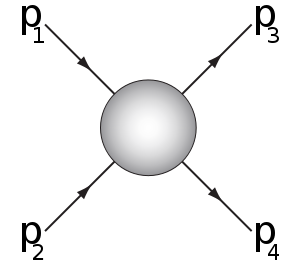
\includegraphics[width=0.2\textwidth]{Mandelstam.png}
\caption{V tomto diagrame častice s $p_1$ a $p_2$ prichádzajú a interagujú zatiaľčo $p_3$ a $p_4$ odchádzajú z interakcie.}
\label{sf1:fig:Mandelstam}
\end{figure}
Každej tejto premennej odpovedá určitá topológia zrážky. Tieto typy odpovedajú rôznym Feynmanovým diagramom. s-kanál, t-kanál, u-kanál, viď obrázok \ref{sf1:fig:Kanaly}.
\begin{figure}[!h]
\centering
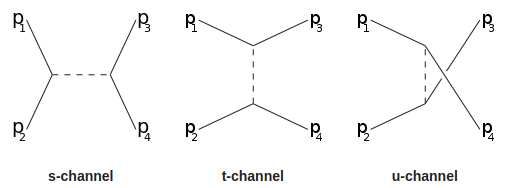
\includegraphics[width=0.6\textwidth]{Kanaly.png}
\caption{s, t, u -kanály. s-kanál je jediný spôsob, akým môžu byť objavené rezonancie a nové nestabilné častice za predpokladu, že ich životnosť je dostatočne dlhá a že sú priamo zistiteľné. t-kanál predstavuje proces, v ktorom častica 1 emituje intermediálnu časticu a stáva sa konečnou časticou 3, zatiaľ čo častica 2 absorbuje intermediálnu časticu a stáva sa 4. Pre u-kanál zameníme v t-kanály len 3 a 4. 
}
\label{sf1:fig:Kanaly}
\end{figure}
\newline
V relativistickej limite zanedbáme hmotnosti oproti hybnosti $p^2 >>> (m_0c^2)^2$.

Suma Mandelstamových premenných nám dá sumu hmotnosti častíc. $$s+t+u=m_1^2+m_2^2+m_3^2+m_4^2$$\newline
\textbf{Lorentzovské transformácie}\par
Uvažujme dve kartézske vztažné sústavy $S$ a $S^{\prime}$, tak že ich počiatky splívajú v čase $t=t^{\prime}=0$. Súradnicové osy oboch sústav sú vzájomne rovnobežné a pohybujú sa tak, že sústava $S$ (kľudová) zostava v pokoji a sústava $S^{\prime}$ sa vzhľadom na $S$ pohybuje rýchlosťou $v$ v kladnom smere osy $x$. Lorentzové transformácie potom sú 
\begin{equation} 
x^{\prime}=\frac{x-vt}{\sqrt{1-\frac{v^2}{c^2}}},\hspace{0.3cm} y^{\prime}=y,\hspace{0.3cm} z^{\prime}=z,\hspace{0.3cm} t^{\prime}=\frac{t-\frac{vx}{c^2}}{\sqrt{1-\frac{v^2}{c^2}}},
\end{equation}
kde $\beta=v/c$ a $c$ je rýchlosť svetla vo vákuum. Pre transformácie energie a hybnosti z jednej do druhej sústavy dostávame 
\begin{equation}
E^{\prime]}=\frac{E-p_xv}{\sqrt{1-\frac{v^2}{c^2}}}, \hspace{0.8cm} p_x^{\prime}=\frac{p_x-\frac{vE}{c^2}}{\sqrt{1-\frac{v^2}{c^2}}}
\end{equation}\newline
\textbf{Kinematika zrážkových procesov}\par
Experimentálne zrážkové procesy: experiment s pevným terčom, experiment s naproti idúcimi zväzkami, viď obrázok \ref{sf1:fig:Zrazky}.
\begin{figure}[!h]
\centering
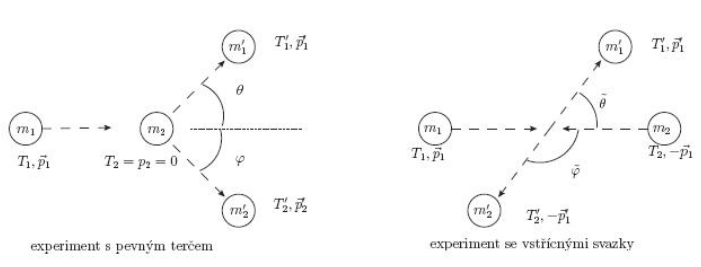
\includegraphics[width=0.8\textwidth]{Zrazky.png}
\caption{Rôzne druhy zrážkových procesov. Vľavo Lab frame a vpravo CMS frame.}
\label{sf1:fig:Zrazky}
\end{figure}
Sústavy sú pred aj po interakcii izolovane. Oblasť, kde sa častice stretnú a interagujú sa nazýva $interakčná$ $oblasť$. Mimo tuto oblasť sa častice pohybujú voľne (reálne je sila interakcie zanedbateľne menšia ako pre oblasť interakcie). Budeme používať nasledovne značenie veličín: pred interakciou budu veličiny bez čiarky a po zrážke s čiarkou.

Zákony zachovania energie a celkovej hybnosti izolovanej sústavy môžme napísať v tvare: $E=E^{\prime}$ a $\vec{P}=\vec{P}^{\prime}$. Podľa produktov rozlišujeme následujúce dva druhy interakcii
\begin{itemize}
	\item \textbf{Pružný rozptyl}: nemenia sa pokojové hmotnosti ani typy častíc po interakcii. Zo zákona zachovania energie plynie, že celková kinetická energia sa zachováva.
	\item \textbf{Nepružný rozptyl}: pri interakcii sa menia hmotnosti zúčastnených častíc. Veličinu $Q=[(m_1+m_2)^2-(m_1^{\prime}+m_2^{\prime})^2]=(M-M^{\prime})^2$ nazývame energia interakcie. Zo zákona zachovania plynie $T^{\prime}=T+Q$. Pre nepružnú interakciu je $Q$ nerovné nule a naopak pre pružnú zrážku je to $Q$ rovné nule. 
\end{itemize}
\textbf{Súradnicové systémy}\par
\begin{itemize}
	\item \textbf{Laboratórna sústava} - táto sústava je pevne spojená s detektorom. Jej použitie nie je vždy vhodne, keďže vzťahy popisujúce interakciu sú v nej dosť zložite. V tejto sústave sa merajú hlavne experimenty s pevným terčom. Avšak, nemusí to byť vždy sústava spojené s detektorom. Používa sa aj laboratórna sústava spojená s nejakou časticou, s ktorou ma druhá častica interagovať.
	\item \textbf{Ťažisková sústava (CMS)} - táto sústava je v pokoji. Zaujíma nás len relatívny pohyb častíc. Celková hybnosť častíc je rovná nule, čo dosť môže zjednodušiť výpočet.
	\item \textbf{Terčiková sústava} - sústava v ktorej je hybnosť terča nulová.
	\item \textbf{Sústava zväzku} - sústava, v ktorej je hybnosť zväzku nulová.
	\item \textbf{Coliding beam frame} - sústava, v ktorej sa zväzky zrážajú pod uhlom $\theta$.
\end{itemize}
Kinetickú energiu v laboratórnej sústave je možne rozdeliť na časť, ktorá prislúcha translačnému pohybu sústavy častíc - (kinetickú energiu ťažiska) a časť, ktorá prislúcha relatívnemu pohybu častíc-(kinetická energia v ťažiskovej sústave). Kinematické vzťahy v ťažiskovej sústave sa vyznačujú maximálnou symetriou, čo je jednoduchšie na výpočty. Vzhľadom k tomu, že väčšina experimentálnych výsledkov je získaná v laboratórnej sústave, je nutne medzi ťažiskovou a laboratórnou sústavou prechádzať.

Zapíšeme zákon zachovania hybnosti, zákon zachovania energie a rýchlosti ťažiska v laboratórnej sústave
\begin{equation}
\begin{gathered}
\vec{p_1}+\vec{p_2}=\vec{p_1}^{\prime}+\vec{p_2}^{\prime} \\
T_1+T_2=T_1^{\prime}+T_2^{\prime} \\
\vec{v}_T=\frac{m_1\vec{v}_1+m_2\vec{v}_2}{m_1+m_2}.
\end{gathered}
\end{equation}
Teraz uvedieme zákony zachovania a rýchlosť ťažiska v ťažiskovej sústave
\begin{equation}
\begin{gathered}
\tilde{\vec{p}}_1+\tilde{\vec{p}}_2=\tilde{\vec{p}}_1^{\prime}+\tilde{\vec{p}}_2^{\prime}=0 \\
\tilde{T}_1+\tilde{T}_2=\tilde{T}_1^{\prime}+\tilde{T}_2^{\prime} \\
\vec{v}_T=0.
\end{gathered}
\end{equation}
Z čoho plynie $$ \lvert \tilde{\vec{p}}_1 \rvert=\lvert \tilde{\vec{p}}_2 \rvert=\lvert \tilde{\vec{p}}_1 \rvert=\lvert \tilde{\vec{p}}_2  \rvert, \hspace{0.3cm} \tilde{\vec{v}}_1=\tilde{\vec{v}}_1^{\prime}, \hspace{0.3cm} \tilde{\vec{v}}_2=\tilde{\vec{v}}_2^{\prime}, \hspace{0.3cm} \tilde{T}_1=\tilde{T}_1^{\prime}, \hspace{0.3 cm} \tilde{T}_2=\tilde{T}_2^{\prime}. $$
Za predpokladu, že je v laboratórnej sústave terčiková častica v pokoji ($p_2=0, T_2=0$), potom platí
\begin{equation}
\begin{gathered}
\tilde{\vec{v}}_1=\vec{v}_1-\vec{v}_T=\vec{v}_1-\frac{m_1\vec{v}_1+m_2\vec{v}_2}{m_1+m_2}=\frac{m_2}{m_1+m_2}\vec{v}_1\rightarrow \tilde{\vec{p}}_1=\mu \vec{v}_1 \\
\tilde{\vec{v}}_2=\vec{v}_2-\vec{v}_T=\vec{v}_2-\frac{m_1\vec{v}_1+m_2\vec{v}_2}{m_1+m_2}=-\frac{m_1}{m_1+m_2}\vec{v}_1\rightarrow \tilde{\vec{p}}_2=-\mu \vec{v}_1 \\
\tilde{T}=\tilde{T}_1+\tilde{T}_2=\frac{\tilde{p}_1^2}{2m_1}+\frac{\tilde{p}_2^2}{2m_2}=\frac{1}{2}\mu v_1^2=\frac{m_2}{m_1+m_2}T_1
\end{gathered}
\end{equation}
kde $\mu=\frac{m_1m_2}{m_1+m_2}$ je redukovaná hmotnosť. Toto sú vzťahy prechodu medzi ťažiskovou a laboratórnou sústavou.

\section{Kinematické premenné}
Uvažujeme že $c=\hbar=1$.\newline
Majme proces $a+b\rightarrow c+X$, kde $X$ sú nešpecifikované častice. Časticu $c$ môžme považovať za dcérsku časticu od častice $a$ alebo $b$. Zrážku častíc budeme uvažovať v sústave, kde zväzok častíc $a$ nalietava v smere osi $z$ na terč tvorený časticami $b$.\newline
Označme 
\begin{equation}
\begin{gathered}
p_a=(E_a,\vec{p}_{Ta},p_{za})\hspace{0.6cm} 4-impulz\hspace{0.2cm} nalietavajucej \hspace{0.2cm} castice \\
p_b=(E_b,\vec{p}_{Tb},p_{zb})\hspace{0.6cm} 4-impulz\hspace{0.2cm} tercikovej \hspace{0.2cm} castice,
\end{gathered}
\end{equation}
kde sme zaviedli tkz. priečnu hybnosť, ktorá je definovaná ako $p_T=p\sin(\theta)$, kde $\theta$ je uhol rozptylu.

Hľadáme premenné, ktoré sú zložené zo zložiek 4-impulzu častice (ktorú meriame) a majú nejakú špeciálnu vlastnosť pri Lorentzovskej transformácii (čo nám veľmi zjednoduší popis). Pre detekovanú dcérsku časticu $c$ definujeme
\begin{equation}
\begin{gathered}
c_+=E_c+p_{zc} \hspace{0.6cm} forward \hspace{0.2cm} lightcone \hspace{0.2cm} momentum \\
c_-=E_c-p_{zc} \hspace{0.6cm} backward \hspace{0.2cm} lightcone \hspace{0.2cm} momentum.
\end{gathered}
\end{equation}
Pre pomer dvoch lightcone premenných platí (zároveň to je Lorentzovký invariant)
$$ x_{\pm}=\frac{E_c\pm p_{cz}}{E_b\pm p_{bz}} \hspace{0.3cm} 0<x_{\pm}<1, $$ 
kde $x_{\pm}$ je forward (backward) lightcone premenná častica $c$ vzhľadom k častici $b$.

Rovnako by sme mohli zaviesť $x_{\pm}$ vzhľadom na časticu $a$ pretože nie vždy je možne povedať, ktorá častica je materskou časticou. Pokiaľ skúmame experiment, ktorý produkuje častice v jednom preferovanom smere, berieme obvykle len jednu z lightcone premenných, druhá sa nepoužíva.\newline

\textbf{Rapidita}\par
Rapidita je bezrozmerná fyzikálna veličina, ktorá je mierou pohybu priestorom, podobne ako rýchlosť. Zatiaľčo rýchlosť objektov je podľa špeciálnej teórie relativity zhora omedzená rýchlosťou svetla vo vákuu $c$, rapidita môže byť ľubovolne veľká. Pre objekty v pokoji má hodnotu 0 a pre pomalé objekty je priamo úmerná rýchlosti. Keď sa rýchlosť objektov približuje k rýchlosti svetla $c$, rastie rapidita nad všetky medze. Je definovana nasledovne $$ y=\frac{1}{2}\ln\bigg( \frac{E+p_z}{E-p_z} \bigg)=\frac{1}{2}\ln\bigg( \frac{x_+}{x_-} \bigg), $$
v nerelativisticke limite $y\rightarrow \beta$. Rapidita nie je lorentzovsky invariant, ale transformuje sa ako $\tilde{y}=y-y_{\beta}$ kde $y_{\beta}$ je rýchlosť pohybujúcej sa vzťažnej sústavy $S^{\prime}$.

Ďalej platí
\begin{equation}
\begin{gathered}
E=m_T\cosh(y) \\
p_z=m_T\sinh(y),
\end{gathered}
\end{equation}
kde veličina $m_T$ je tzv. priečna hmotnosť a je definovaná nasledujúcim spôsobom
$$ m^2=E^2-p^2=E^2-p_z^2-p_T^2 \hspace{0.2cm} \rightarrow \hspace{0.2cm} E^2-p^2_z=m^2+p^2_T=m^2_T. $$\newline
\newpage
\textbf{Pseudorapidita}\par
Jej výhodou je oproti rapidite v tom, že stačí jedna premenná pre jej definíciu - uhol výletu. Pseudorapidita je definovaná následovne
$$ \eta=-\ln\bigg( \tan\frac{\theta}{2}  \bigg) = \frac{1}{2}\ln \bigg( \frac{\lvert \vec{p} \rvert+p_z}{\lvert \vec{p} \rvert-p_z} \bigg), $$
kde uhol $\theta$ je uhol medzi hybnosťou častice $\vec{p}$ a osou zväzku. V druhej časti vzťahu môžme vidieť, že pre veľké hybnosti (resp. male hmotnosti) rapidita a pseudorapidita splývajú ($p\approx E$).
\begin{figure}[!h]
\centering
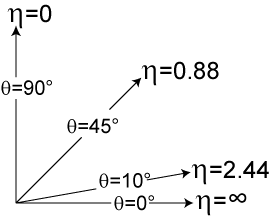
\includegraphics[width=0.3\textwidth]{Pseudorapidity.png}
\caption{Tu môžme vidieť ako sa pseudorapidita mení s uhlom $\theta$.}
\label{sf1:fig:Pseudorapidity}
\end{figure}
\newline

\textbf{Feynmanova promenna}\par
Bola zavedená pri štúdiu vysoko-energetických zrážok hadrónov pre popis elementárnej interakcie na kvarkovej úrovni. Je definovaná vzťahom $$ x_F=\frac{\tilde{p}_z}{\tilde{p}_z^{max}}. $$
Feynmanová premenná je obvykle definovaná v sústave, v ktorej sa častica pohybuje s nekonečnou hybnosťou (infinite momentum frame). Je tomu tak preto, lebo v kvantovej mechanike nie je operator počtu častíc invariantný voči prechodu z jednej sústavy do druhej, a tak počet častíc, ktoré pozorujeme pri lete vysoko-energetickej častice, závisí na sústave, v ktorej proces študujeme. Limitná sústava je potom sústava, kde sa všetky častice pohybujú s nekonečnou hybnosťou, a tak doba života kvantovo vytvorených častíc je nekonečne malá a je tak možne dobre definovať časticové obsadenie sústavy. V tejto sústave môžme ukázať, že $x_F=\frac{2\tilde{p}_z}{\sqrt{s}}.$ Ďalej tiež platí $0<x_F<1$ a pre $E\rightarrow \infty$ mame $x_F=1$.\newline

\textbf{Bjorkenova promenna}\par
Je to veličina, ktorá je definovaná následovne $$ x=\frac{Q^2}{2(p_2\cdot q)}, $$ kde $Q^2=-q^2$. Na obrázku \ref{sf1:fig:Bjorken} sú znázornene jednotlive 4-impulzy vyskytujúce sa v tejto premenne.
\begin{figure}[!h]
\centering
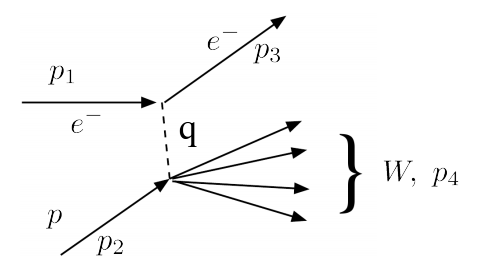
\includegraphics[width=0.6\textwidth]{Bjorken.png}
\caption{Rozptyl elektrónu na protóne.}
\label{sf1:fig:Bjorken}
\end{figure}
Podľa obrázka mame
$$ p_4^2=M_W^2=(q+p_2)^2=q^2+2qp_2+p_2^2=-Q^2+2qp_2+M_p^2\rightarrow Q^2=2qp_2+M_p^2-M_W^2,$$
keďže je $M_p$ hmotnosť protónu, ktorý je najľahší baryón, a $M_W$ hmotnosť akéhokoľvek iného baryónu tak hodnota $Q^2$ nebude nikdy väčšia ako $2qp_2$.
Potom mame pre neelastický rozptyl: $0<x<1$, zatiaľčo pre elastický rozptyl $x=1$.

\end{document}